
\section{network terminology}

\subsection{nodes / links / internetworks}

\usetikzlibrary{arrows.meta,calc,shapes}
\providecommand{\computer}{%
    
\includegraphics[width=1cm]{../common/Noun_project_216.pdf}
}
\providecommand{\switch}{%
    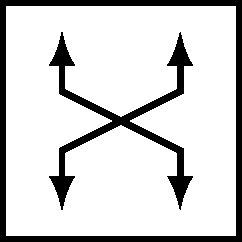
\includegraphics[width=0.9cm]{../common/fig-switch.pdf}
}
\providecommand{\router}{%
    
\includegraphics[width=0.9cm]{../common/fig-router.pdf}
}


\begin{frame}\frametitle{networks / hosts aka end systems}
\myalttextD{%
\begin{tikzpicture}
\tikzset{
    connect/.style={draw,very thick,Latex-Latex},
    computer/.style={inner sep=0mm,outer sep=0mm,beameralt=<4>{label={[font=\small,label distance=0mm,text=red]south:`host'}},execute at begin node={\computer}},
}
\node[
      cloud,draw,very thick,aspect=2,
      minimum width=4cm,minimum height=3cm,
      beameralt=<2-3>{draw=red,fill=red!10,label={[text=red]center:`network'}},
     ] (net-cloud) at (0,0) {};
\foreach \x/\d in {0/5cm,45/4cm,90/3cm,135/4cm,180/5cm,225/4cm,270/3cm,315/4cm} {
    \node[computer] (c-\x) at (\x:\d) {};
    \draw[connect] (net-cloud) -- (c-\x);
}
\coordinate (box loc) at (4cm, 3.5cm);
\tikzset{
    explain box/.style={
        overlay,draw=red, align=left, very thick, anchor=north west
    },
}
\begin{visibleenv}<2>
\node[explain box] at (box loc) {
    \textit{networks} connect \\
    computers 
};
\end{visibleenv}
\begin{visibleenv}<3>
\node[explain box] at (box loc) {
    `cloud' represents \\
    any network \\
    (whether local or not) \\
    \small iconography predates \\
    \small `cloud computing'
};
\end{visibleenv}
\begin{visibleenv}<4>
\node[explain box] at (box loc) {
    computers on edge \\
    of network called \\
    \textit{hosts} or \textit{end systems} \\
    \small (even if also `servers')
};
\end{visibleenv}
\end{tikzpicture}
}{
Picture showing computers connected via lines with arrowheads on both ends to a cloud.
}{
Same diagram as previous slide. The cloud is labeled as a `network' and a box reads ``networks connect computers''.
}{
Same diagram as previous slide. The cloud is labeled as a `network' and a box reads ``cloud represents any network (whether local or not). Iconography predates cloud computing.''
}{
Same diagram as previous slide. The computers are labeled `hosts' and a box reads ``computers on edge of network called hosts or end systems (even if also `severs').''
}
\end{frame}

\begin{frame}\frametitle{direct connections?}
\myalttext{%
\begin{tikzpicture}
\tikzset{
    connect/.style={draw,very thick,Latex-Latex},
    computer/.style={inner sep=0mm,outer sep=0mm,execute at begin node={\computer}},
}
\foreach \x/\d in {0/5cm,45/4cm,90/3cm,135/4cm,180/5cm,225/4cm,270/3cm,315/4cm} {
    \node[computer] (c-\x) at (\x:\d) {};
    \foreach \y in {0,45,90,135,180,225,270,315} {
        \ifnum \x = \y
            \relax
        \else
            \draw[connect] (c-\x) -- (c-\y);
        \fi
    }
}
\end{tikzpicture}
}{%
Picture showing 8 computers connected to each other via 56 lines (one for each pair of computers).
}
\end{frame}

\begin{frame}\frametitle{shared medium: radio?}
\myalttext{%
\begin{tikzpicture}
\tikzset{
    connect/.style={draw,very thick,Latex-Latex},
    computer/.style={inner sep=0mm,outer sep=0mm,execute at begin node={\computer}},
}
\foreach \x/\d in {0/5cm,45/4cm,90/3cm,135/4cm,180/5cm,225/4cm,270/3cm,315/4cm} {
    \node[computer] (c-\x) at (\x:\d) {};
%    %\begin{visibleenv}<2->
    \pgfmathsetmacro\oppX{\x+180}
    \path (c-\x.\oppX) -- ++(\oppX:0.1) coordinate (c-\x-wifi);
    \foreach \y in {0.2,0.35,0.5} {
        \draw[ultra thick] (c-\x-wifi) ++ (\oppX-50:\y) arc (\oppX-50:\oppX+50:\y);
    }
%    %\end{visibleenv}
}
\end{tikzpicture}
}{%
Picture showing the same 8 computers with wifi-like symbols indicating they communicate via radio.%
}
\end{frame}

\begin{frame}\frametitle{shared medium: wires}
\myalttextC{%
\begin{tikzpicture}
\tikzset{
    connect/.style={draw,very thick,arrows={Latex-Circle[width=0.3cm,length=0.3cm]},
        beameralt=<2>{arrows={Latex-Circle[width=0.3cm,length=0.3cm,red]}}},
    computer/.style={inner sep=0mm,outer sep=0mm,execute at begin node={\computer}},
}
\draw[line width=1mm] (-5,-1.5) coordinate (wire start) -- (5, 1.5) coordinate (wire end);
\foreach \x/\d in {0/5cm,45/4cm,90/3cm,135/4cm,180/5cm,225/4cm,270/3cm,315/4cm} {
    \node[computer] (c-\x) at (\x:\d) {};
    \coordinate (connect-\x) at ($(wire start)!(c-\x.center)!(wire end)$);
    \draw[connect] (c-\x) -- (connect-\x) -- ([turn]0:.1cm);
}
\begin{visibleenv}<2-3>
\node[anchor=north west,fill=white,draw=black,thick,label={[font=\tiny]south:Ali at gwc.org.uk / Alistair1978 via Wikimedia commons / CC-BY-SA 2.5}] 
    (thicknet) at (4, 3.5) {
    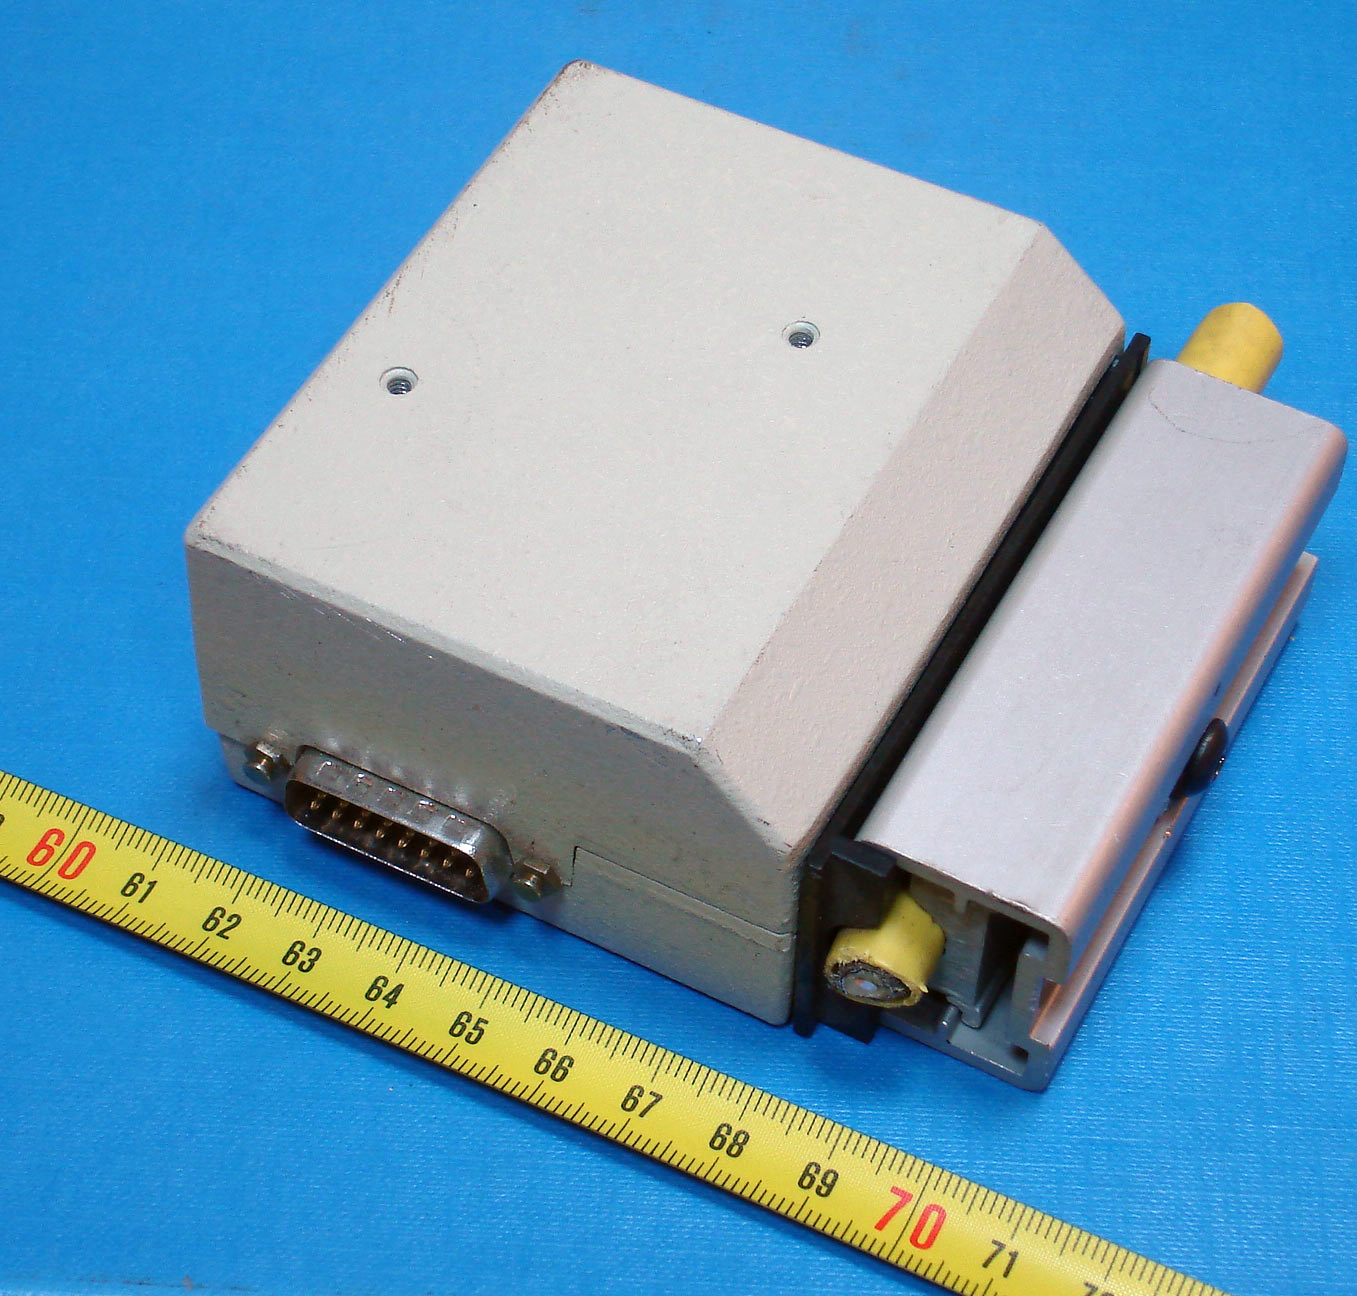
\includegraphics[width=4cm]{../intro/ThicknetTransceiver.jpeg}
};
\end{visibleenv}
\begin{visibleenv}<3>
\node[fill=white,draw=black,thick,anchor=north west] at ([yshift=-0.75cm]thicknet.south west) {
    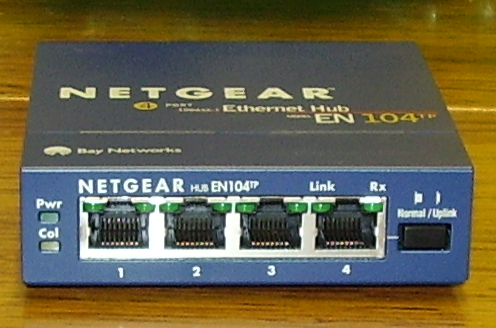
\includegraphics[width=4cm]{../intro/4_port_netgear_ethernet_hub}
};
% FIXME: also fiber splitter
\end{visibleenv}
\end{tikzpicture}
}{
Picture showing 8 computers connected via vertical lines to a single horizontal line representing a wire.
}{
Same picture as before with the connection between the vertical lines and horizontal lines highlighted, and a picture of a Thicknet transciever, a device
that screws into coax cable to provide an electrical connection.
}{
Same picture as before with the addition of a picture of a 4-port Ethernet hub --- a Netgear-branded box with four RJ-45 ports.
}
\end{frame}

\begin{frame}\frametitle{switches / nodes / links}
\begin{tikzpicture}
\tikzset{
    computer/.style={inner sep=0mm,outer sep=0mm,execute at begin node={\computer},beameralt=<3>{fill=red!10}},
    switch/.style={inner sep=0mm,outer sep=0mm,execute at begin node={\switch},
                   beameralt=<2>{
                       fill=red!10,
                        label={[font=\small,label distance=0mm,text=red]south:`switch'}
                   },
                   beameralt=<3>{fill=red!10}},
    connect/.style={draw,very thick,Latex-Latex,beameralt=<4>{red}},
    connect big/.style={draw,ultra thick,Latex-Latex,beameralt=<4>{red}},
}
\node[
      cloud,draw,opacity=0.25,very thick,aspect=2,
      minimum width=7cm,minimum height=4cm,
     ] (net-cloud) at (0,0) {};
\foreach \x/\d in {0/5cm,45/4cm,90/3cm,135/4cm,180/5cm,225/4cm,270/3cm,315/4cm} {
    \node[computer] (c-\x) at (\x:\d) {};
}
\node[switch] (s1) at (2,-0.5) {};
\node[switch] (s2) at (-1,0.5) {};
\node[switch] (s3) at (0,-1) {};
\draw[connect] (c-0) -- (s1);
\draw[connect] (c-45) -- (s1);
\draw[connect] (c-315) -- (s1);
\draw[connect] (c-90) -- (s2);
\draw[connect] (c-135) -- (s2);
\draw[connect] (c-180) -- (s2);
\draw[connect] (c-225) -- (s3);
\draw[connect] (c-270) -- (s3);
\draw[connect big] (s1) -- (s2);
\draw[connect big] (s1) -- (s3);
\coordinate (box loc) at (4cm, 4.5cm);
\begin{visibleenv}<2>
\node[overlay,draw=red, align=left, very thick, anchor=north west] at (box loc) {
    hosts directly connected to \\
    \textit{\myemph{switches}} \\
    that implement network \\
    ~ \\
    (more efficiently than \\
    shared medium)
};
\end{visibleenv}
\begin{visibleenv}<3>
\node[overlay,draw=red, align=left, very thick, anchor=north west] at (box loc) {
    machines on network \\
    (hosts, switches, \ldots) \\
    called \textit{\myemph{nodes}}
};
\end{visibleenv}
\begin{visibleenv}<4>
\node[overlay,draw=red, align=left, very thick, anchor=north west] at (box loc) {
    nodes connected by \\
   \textit{\myemph{links}} \\
    ~ \\
    (implemented by wires \\
    or radio or \ldots)
};
\end{visibleenv}
\end{tikzpicture}
\end{frame}

% FIXME: picture of physical switch

\begin{frame}{routers / internetwork}
\begin{tikzpicture}
\tikzset{
    computer/.style={inner sep=0mm,outer sep=0mm,execute at begin node={\computer}},
    switch/.style={inner sep=0mm,outer sep=0mm,execute at begin node={\switch}},
    router/.style={inner sep=0mm,outer sep=0mm,execute at begin node={\router},circle,
        beameralt=<2>{fill=red!10}},
    connect/.style={draw,very thick,Latex-Latex},
    connect big/.style={draw,ultra thick,Latex-Latex},
}
\node[
      cloud,draw,opacity=0.25,very thick,aspect=2,
      minimum width=3cm,minimum height=2cm,
     ] (net-1) at (-1,1) {};
\node[
      cloud,draw,opacity=0.25,very thick,aspect=2,
      minimum width=3cm,minimum height=2cm,
     ] (net-2) at (3,0) {};
\node[
      cloud,draw,opacity=0.25,very thick,aspect=2,
      minimum width=3cm,minimum height=2cm,
     ] (net-3) at (-2,-4) {};
\node[
      cloud,draw,opacity=0.25,very thick,aspect=2,
      minimum width=3cm,minimum height=2cm,
     ] (net-4) at (2,-3) {};

\node[
      cloud,draw,opacity=0.25,very thick,aspect=2,
      minimum width=3cm,minimum height=2cm,
     ] (net-5) at (6,-4) {};
% FIXME: routers
\node[router] (r1) at (-2, -1.5) {};
\draw[connect big] (r1) -- (net-1);
\draw[connect big] (r1) -- (net-2);
\draw[connect big] (r1) -- (net-3);
\node[router] (r2) at (5, -2) {};
\draw[connect big] (r2) -- (net-4);
\draw[connect big] (r2) -- (net-5);
\draw[connect big] (r2) -- (net-2);
\node[router] (r3) at (3, -5) {};
\draw[connect big] (r3) -- (net-3);
\draw[connect big] (r3) -- (net-5);
\coordinate (box loc) at (6, 2);
\tikzset{
    explain box/.style={
        overlay,draw=red, align=left, very thick, anchor=north west
    },
}
\begin{visibleenv}<2>
\node[explain box] at (box loc) {
    \textit{\myemph{routers}} or \textit{\myemph{gateways}} \\
    connect networks
};
\end{visibleenv}
\begin{visibleenv}<3>
\node[explain box] at (box loc) {
    connected networks \\
    form \textit{\myemph{internetwork}}
    ~ \\
    (example: the Internet)
};
\end{visibleenv}
\end{tikzpicture}
\end{frame}



\subsection{flows}

\usetikzlibrary{arrows.meta,calc,patterns,shapes}
\providecommand{\computer}{%
    
\includegraphics[width=1cm,alt={computer}]{../common/Noun_project_216.pdf}
}
\providecommand{\switch}{%
    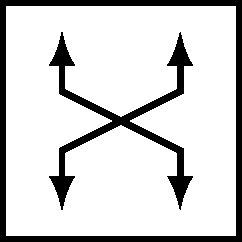
\includegraphics[width=0.9cm,alt={switch}]{../common/fig-switch.pdf}
}
\providecommand{\bigswitch}{%
    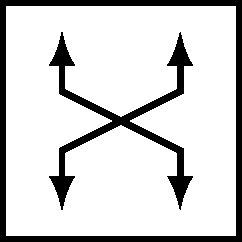
\includegraphics[width=1.4cm,alt={switch}]{../common/fig-switch.pdf}
}
\providecommand{\router}{%
    
\includegraphics[width=0.9cm,alt={router}]{../common/fig-router.pdf}
}



\begin{frame}\frametitle{flows / packets}
\begin{tikzpicture}
\tikzset{
    connect one/.style={draw,very thick,-Latex},
    computer/.style={inner sep=0mm,outer sep=0mm,execute at begin node={\computer}},
    switch/.style={inner sep=0mm,outer sep=0mm,execute at begin node={\switch}},
    big switch/.style={inner sep=0mm,outer sep=0mm,execute at begin node={\bigswitch}},
    packet/.style={minimum width=.4cm,minimum height=0.2cm,inner sep=0mm,outer sep=0mm,draw},
    packet lg/.style={minimum width=.6cm,minimum height=0.2cm,inner sep=0mm,outer sep=0mm,draw},
    c1c2/.style={fill=violet!40,draw=black,thin,slidealt=<2>{thick,draw=red}},
}
\node[computer] (c1) at (-5, 1) {};
\node at (c1) {1};
\node[big switch] (s1) at (-2,-.5) {};
\node[big switch] (s2) at (2,.5) {};
\node[computer] (c2) at (6, 2) {};
\node at (c2) {2};
\draw[connect one] (c1) -- (s1)
    node[above=0.05cm,sloped,packet,c1c2,pos=0.1] {}
    node[above=0.05cm,sloped,packet lg,c1c2,pos=0.5] {}
    node[above=0.05cm,sloped,packet,c1c2,pos=0.8] {};
\draw[connect one] (s1) -- (s2)
    node[above=0.05cm,sloped,packet,c1c2,pos=0.3] {}
    node[above=0.05cm,sloped,packet,c1c2,pos=0.8] {};
\draw[connect one] (s2) -- (c2)
    node[above=0.05cm,sloped,packet,c1c2,pos=0.2] {}
    node[above=0.05cm,sloped,packet lg,c1c2,pos=0.6] {};
\node[packet,c1c2,anchor=north east] at ([yshift=-.1cm,xshift=-.1cm]s1.north east) {};
\node[packet lg,c1c2,anchor=north east] at ([yshift=-.3cm,xshift=-.1cm]s1.north east) {};
%
\node[packet,c1c2,anchor=north east] at ([yshift=-.1cm,xshift=-.1cm]s2.north east) {};
\node[packet,c1c2,anchor=north east] at ([yshift=-.3cm,xshift=-.1cm]s2.north east) {};
\node[packet,c1c2,anchor=north east] at ([yshift=-.5cm,xshift=-.1cm]s2.north east) {};
\coordinate (box loc) at (-4, -1.5);
\tikzset{
    explain box/.style={
        overlay,draw=red, align=left, very thick, anchor=north west,at=(box loc)
    },
}
\begin{visibleenv}<1>
\node[explain box] {
    \textit{\myemph{flow}} of data between two machines \\
    ~ \\
    \textit{flow} is very general term \\
    will depend on context how it relates to \\
    connections, sockets, etc.
};
\end{visibleenv}
\begin{visibleenv}<2>
\node[explain box] {
    \textit{\myemph{flow}} of data between two machines \\
    ~ \\
    possibly divided up into pieces, \\
    called \textit{\myemph{packets}}, \textit{\myemph{frames}}, \textit{\myemph{segments}} \\
    (which name is best depends on context)
};
\end{visibleenv}
\end{tikzpicture}
\end{frame}

\begin{frame}\frametitle{(de)multiplexing}
\begin{tikzpicture}
\tikzset{%
    connect one/.style={draw,very thick,-Latex},
    connect one lg/.style={draw,line width=1mm,-Latex},
    connect one sm/.style={draw,thick,-Latex},
    computer/.style={inner sep=0mm,outer sep=0mm,execute at begin node={\computer}},
    switch/.style={inner sep=0mm,outer sep=0mm,execute at begin node={\switch}},
    big switch/.style={inner sep=0mm,outer sep=0mm,execute at begin node={\bigswitch}},
    packet/.style={minimum width=.4cm,minimum height=0.2cm,inner sep=0mm,outer sep=0mm,draw},
    packet lg/.style={minimum width=.6cm,minimum height=0.2cm,inner sep=0mm,outer sep=0mm,draw},
    c1c2/.style={fill=violet!40,draw=black,thin},
    c3c4/.style={pattern=checkerboard,pattern color=green!70,draw=black,thin},
    buffer 1/.style={slidealt=<5>{draw=red,thick},slidealt=<8>{draw=red,thick}},
    buffer 2/.style={slidealt=<5>{draw=red,thick}},
}
\node[computer] (c1) at (-5, 1) {};
\node at (c1) {1};
\node[big switch,slidealt=<3-4>{fill=red!10},slidealt=<6>{fill=red!10}] (s1) at (-2,-.5) {};
\node[big switch,slidealt=<3-4>{fill=red!10}] (s2) at (2,.5) {};
\node[computer] (c2) at (6, 2) {};
\node at (c2) {2};
\node[computer] (c3) at (-5, -1) {};
\node at (c3) {3};
\node[computer] (c4) at (6, 0) {};
\node at (c4) {4};
\draw[connect one] (c3) -- (s1)
    node[above=0.05cm,sloped,packet lg,c3c4,pos=0.2] {}
    node[above=0.05cm,sloped,packet,c3c4,pos=0.7] {};
\draw[connect one] (c1) -- (s1)
    node[above=0.05cm,sloped,packet,c1c2,pos=0.1] {}
    node[above=0.05cm,sloped,packet lg,c1c2,pos=0.5] {}
    node[above=0.05cm,sloped,packet,c1c2,pos=0.8] {};
\draw[connect one,slidealt={<2>{draw=red,ultra thick}}] (s1) -- (s2)
    node[above=0.05cm,sloped,packet,c1c2,pos=0.3] {}
    node[above=0.05cm,sloped,packet,c3c4,pos=0.6] {}
    node[above=0.05cm,sloped,packet,c1c2,pos=0.8] {};
\draw[connect one sm] (s2.north east) -- (c2)
    node[above=0.05cm,sloped,packet,c1c2,pos=0.2] {}
    node[above=0.05cm,sloped,packet lg,c1c2,pos=0.6] {};
\draw[connect one sm] (s2.south east) -- (c4)
    node[above=0.05cm,sloped,packet,c3c4,pos=0.2] {}
    node[above=0.05cm,sloped,packet lg,c3c4,pos=0.6] {};
\node[packet,c3c4,buffer 1,anchor=north east] at ([yshift=-.1cm,xshift=-.1cm]s1.north east) {};
\node[packet,c1c2,buffer 1,anchor=north east] at ([yshift=-.3cm,xshift=-.1cm]s1.north east) {};
\node[packet lg,c1c2,buffer 1,anchor=north east] at ([yshift=-.5cm,xshift=-.1cm]s1.north east) {};
\begin{visibleenv}<8>
\node[packet,c3c4,buffer 1,anchor=north east,opacity=0.9,draw=red] at ([yshift=-.7cm,xshift=-.1cm]s1.north east) {};
\node[packet lg,c1c2,buffer 1,anchor=north east,opacity=0.8,draw=red] at ([yshift=-.9cm,xshift=-.1cm]s1.north east) {};
\node[packet,c1c2,buffer 1,anchor=north east,opacity=0.7,draw=red] at ([yshift=-1.1cm,xshift=-.1cm]s1.north east) {};
\node[packet,c1c2,buffer 1,anchor=north east,opacity=0.5,draw=red] at ([yshift=-1.3cm,xshift=-.1cm]s1.north east) {};
\node[packet,c1c2,buffer 1,anchor=north east,opacity=0.3,draw=red] at ([yshift=-1.3cm,xshift=-.1cm]s1.north east) {};
\node[packet,c1c2,buffer 1,anchor=north east,opacity=0.1,draw=red] at ([yshift=-1.5cm,xshift=-.1cm]s1.north east) {};
\end{visibleenv}
\node[packet,c1c2,buffer 2,anchor=north east] at ([yshift=-.1cm,xshift=-.1cm]s2.north east) {};
\node[packet,c1c2,buffer 2,anchor=north east] at ([yshift=-.3cm,xshift=-.1cm]s2.north east) {};
\node[packet,c1c2,buffer 2,anchor=north east] at ([yshift=-.5cm,xshift=-.1cm]s2.north east) {};
\node[packet lg,c3c4,buffer 2,anchor=south east] at ([yshift=.1cm,xshift=-.1cm]s2.south east) {};
\coordinate (box loc) at (-4, -1.5);
\tikzset{%
    explain box/.style={%
        overlay,draw=red, align=left, very thick, anchor=north west,at=(box loc)
    },
}
\begin{visibleenv}<2>
\node[explain box] {%
    two or more flows can \\
    share one or more links
};
\end{visibleenv}
\begin{visibleenv}<3>
\node[explain box] {%
    left switch \textit{\myemph{multiplexes}} the two flows onto one link \\
    right switch \textit{\myemph{demultiplexes}} them to separate them
};
\end{visibleenv}
\begin{visibleenv}<4>
\node[explain box] {%
    this picture: multiplexed by dividing up \textit{time} on link
};
\end{visibleenv}
\begin{visibleenv}<5>
\node[explain box] {%
    switches usually have \textit{\myemph{buffers}} (also called \textit{\myemph{queues}}) \\
    hold waiting packets \\
    ~ \\
    absorbs temporary ``bursts'' where packets come faster \\
    than outgoing link can handle
        % FIXME: diagram of packets coming in over time
};
\end{visibleenv}
\begin{visibleenv}<6-7>
\node[explain box] {%
    incomplete list of causes of `bursts': \\
    ~ \\
    \myemph<6>{multiple unsynchronized flows} \\
    \myemph<7>{fast links produce packets faster for slow can send}
};
\end{visibleenv}
\begin{visibleenv}<8>
\node[explain box] {%
    if buffer full, switch must \textit{\myemph{drop}} packets \\
    will happen eventually if overall rate faster than outgoing link \\
    ~\\
    scenario is called \textit{\myemph{congestion}}
};
\end{visibleenv}
\end{tikzpicture}
\end{frame}

\begin{frame}\frametitle{buffer usage: fast to slow, store + forward}
\begin{tikzpicture}
\tikzset{
    axis/.style={draw,thick,-Latex},
    scale mark/.style={draw,thin},
    scale label/.style={font=\small},
    packet/.style={ultra thick,fill=violet!20},
    y=.6cm
}
\begin{scope} % input
    \begin{scope}[shift={(0.1, 0)}]
        \clip (0, 0) rectangle (12.5, 3.2);
        \draw[packet] (0, 0) coordinate (A recv start) rectangle (2, 3) node[midway] {packet A};
        \draw[packet] (2, 0) rectangle (4, 3) node[midway] {packet B};
        \draw[packet] (4, 0) rectangle (6, 3) node[midway] {packet C};
        \draw[packet] (10, 0) rectangle (12, 3) node[midway] {packet D};
    \end{scope}
    \draw[axis] (0, 0) -- ++ (12.5, 0);
    \draw[axis] (0, 0) -- ++ (0, 3.3)
        node[midway,left=.5cm,align=right] { input };
    \draw[scale mark] (0, 3) -- ++ (.25, 0) node[pos=0,left,scale label] {capacity};
\end{scope} 
\begin{scope}[shift={(0, -5)}]% buffer usage
    \begin{scope}
        \clip (0,0) rectangle (12.5, 4);
        \draw[violet, ultra thick] (0, 0) -- (0.1, 0) -- (0.1, 1) -- (2.1, 1) -- (2.1, 2) -- (4.1, 2) -- (4.1, 3)
            -- (5.1, 3) -- (5.1, 2) -- (8.1, 2) -- (8.1, 1) -- (10.1, 1) -- (10.1, 2) -- 
            (11.1, 2) -- (11.1, 1) -- (14, 1);
    \end{scope}
    \draw[axis] (0, 0) -- ++ (12.5, 0);
    \draw[axis] (0, 0) -- ++ (0, 4.3)
    node[midway,left=.5cm,align=right] (usage label) { buffer \\ reserved };
    \node[font=\small,anchor=north,align=center] at (usage label.south) {
        packets
    };
    \draw[scale mark] (0, 1) -- ++ (.25, 0) node[pos=0,left,scale label] {1};
    \draw[scale mark] (0, 2) -- ++ (.25, 0) node[pos=0,left,scale label] {2};
    \draw[scale mark] (0, 3) -- ++ (.25, 0) node[pos=0,left,scale label] {3};
    \draw[scale mark] (0, 4) -- ++ (.25, 0) node[pos=0,left,scale label] {4};

\end{scope}
\begin{scope}[shift={(0, -8)}] % output
    \begin{scope}
        \clip (0, 0) rectangle (12.5, 2.2);
        \begin{scope}[shift={(2.1, 0)}]
            \draw[packet] (0, 0) coordinate (A send start) rectangle (3, 2) node[midway] {packet A};
            \draw[packet] (3, 0) rectangle (6, 2) node[midway] {packet B};
            \draw[packet] (6, 0) rectangle (9, 2) node[midway] {packet C};
            \draw[packet] (10, 0) rectangle (13, 2) node[midway] {packet D};
        \end{scope}
    \end{scope}
    \draw[axis] (0, 0) -- ++ (12.5, 0);
    \draw[axis] (0, 0) -- ++ (0, 2.3)
        node[midway,left=.5cm,align=right] { output };
    \draw[scale mark] (0, 2) -- ++ (.25, 0) node[pos=0,left,scale label] {capacity};
\end{scope}
\begin{visibleenv}<2>
    \draw[draw=red,dotted,ultra thick,Latex-Latex] (A send start) -- ++(-2cm, 0);
    \draw[draw=red,dotted,ultra thick] (A send start) -- ++(0cm, 6cm);
    \draw[draw=red,dotted,ultra thick] ([xshift=-2cm]A send start) -- ++(0cm, 6cm);
    \node[draw=red,ultra thick,align=left,fill=white,anchor=west] at  (2.2, -3) {
        \textit{store and forward} \\
        switch stores whole packet in buffer\\
        then sends it out \\
        ~ \\
        our default in this class
    };
\end{visibleenv}
\end{tikzpicture}
\end{frame}

\begin{frame}\frametitle{buffer usage: fast to slow, cut-through}
\begin{tikzpicture}
\tikzset{
    axis/.style={draw,thick,-Latex},
    scale mark/.style={draw,thin},
    scale label/.style={font=\small},
    packet/.style={ultra thick,fill=violet!20},
    y=.6cm
}
\begin{scope} % input
    \begin{scope}[shift={(0.1, 0)}]
        \clip (0, 0) rectangle (12.5, 3.2);
        \draw[packet] (0, 0) coordinate (A recv start) rectangle (2, 3) node[midway] {packet A};
        \draw[packet] (2, 0) rectangle (4, 3) node[midway] {packet B};
        \draw[packet] (4, 0) rectangle (6, 3) node[midway] {packet C};
        \draw[packet] (10, 0) rectangle (12, 3) node[midway] {packet D};
    \end{scope}
    \draw[axis] (0, 0) -- ++ (12.5, 0);
    \draw[axis] (0, 0) -- ++ (0, 3.3)
        node[midway,left=.5cm,align=right] { input };
    \draw[scale mark] (0, 3) -- ++ (.25, 0) node[pos=0,left,scale label] {capacity};
\end{scope} 
\begin{scope}[shift={(0, -5)}]% buffer usage
    \begin{scope}
        \clip (0,0) rectangle (12.5, 4);
        \draw[violet, ultra thick] (0, 0) -- (0.1, 0) -- (0.1, 1) -- (2.1, 1) -- (2.1, 2) -- 
            (3.6, 2) -- (3.6, 1) -- (4.1, 1) -- (4.1, 2) -- (6.6, 2) -- (6.6, 1) --
            (9.6, 1) -- (9.6, 0) -- (10.1, 0) -- (10.1, 1) -- (13.6, 1) -- (13.6, 0);
    \end{scope}
    \draw[axis] (0, 0) -- ++ (12.5, 0);
    \draw[axis] (0, 0) -- ++ (0, 4.3)
    node[midway,left=.5cm,align=right] (usage label) { buffer \\ reserved };
    \node[font=\small,anchor=north,align=center] at (usage label.south) {
        packets
    };
    \draw[scale mark] (0, 1) -- ++ (.25, 0) node[pos=0,left,scale label] {1};
    \draw[scale mark] (0, 2) -- ++ (.25, 0) node[pos=0,left,scale label] {2};
    \draw[scale mark] (0, 3) -- ++ (.25, 0) node[pos=0,left,scale label] {3};
    \draw[scale mark] (0, 4) -- ++ (.25, 0) node[pos=0,left,scale label] {4};

\end{scope}
\begin{scope}[shift={(0, -8)}] % output
    \begin{scope}
        \clip (0, 0) rectangle (12.5, 2.2);
        \begin{scope}[shift={(0.6, 0)}]
            \draw[packet] (0, 0) coordinate (A send start) rectangle (3, 2) node[midway] {packet A};
            \draw[packet] (3, 0) rectangle (6, 2) node[midway] {packet B};
            \draw[packet] (6, 0) rectangle (9, 2) node[midway] {packet C};
            \draw[packet] (10, 0) rectangle (13, 2) node[midway] {packet D};
        \end{scope}
    \end{scope}
    \draw[axis] (0, 0) -- ++ (12.5, 0);
    \draw[axis] (0, 0) -- ++ (0, 2.3)
        node[midway,left=.5cm,align=right] { output };
    \draw[scale mark] (0, 2) -- ++ (.25, 0) node[pos=0,left,scale label] {capacity};
\end{scope}
\begin{visibleenv}<1>
    \draw[draw=red,dotted,ultra thick] (A send start) -- ++(-.5cm, 0);
    \draw[draw=red,dotted,ultra thick] (A send start) -- ++(0cm, 6cm);
    \draw[draw=red,dotted,ultra thick] ([xshift=-.5cm]A send start) -- ++(0cm, 6cm);
    \node[draw=red,ultra thick,align=left,fill=white,anchor=west] at  (2.2, -3) {
        \textit{cut-through} forwarding \\
        switch sends packet out as it's being received \\
        ~ \\
        uncommon and much more complex to implement
    };
\end{visibleenv}
\end{tikzpicture}
\end{frame}
% FIXME: multiplexing at end hosts


\subsection{muxing/demuxing}


\begin{frame}\frametitle{(de)multiplexing}
\myalttext{
\begin{tikzpicture}
\tikzset{%
    connect one/.style={draw,very thick,-Latex},
    connect one lg/.style={draw,line width=1mm,-Latex},
    connect one sm/.style={draw,thick,-Latex},
    computer/.style={inner sep=0mm,outer sep=0mm,execute at begin node={\computer}},
    switch/.style={inner sep=0mm,outer sep=0mm,execute at begin node={\switch}},
    big switch/.style={inner sep=0mm,outer sep=0mm,execute at begin node={\bigswitch}},
    packet/.style={minimum width=.4cm,minimum height=0.2cm,inner sep=0mm,outer sep=0mm,draw},
    packet lg/.style={minimum width=.6cm,minimum height=0.2cm,inner sep=0mm,outer sep=0mm,draw},
    c1c2/.style={fill=violet!40,draw=black,thin},
    c3c4/.style={pattern=checkerboard,pattern color=green!70,draw=black,thin},
    buffer 1/.style={slidealt=<5>{draw=red,thick},slidealt=<8>{draw=red,thick}},
    buffer 2/.style={slidealt=<5>{draw=red,thick}},
}
\node[computer] (c1) at (-5, 1) {};
\node at (c1) {1};
\node[big switch,slidealt=<3-4>{fill=red!10},slidealt=<6>{fill=red!10}] (s1) at (-2,-.5) {};
\node[big switch,slidealt=<3-4>{fill=red!10}] (s2) at (2,.5) {};
\node[computer] (c2) at (6, 2) {};
\node at (c2) {2};
\node[computer] (c3) at (-5, -1) {};
\node at (c3) {3};
\node[computer] (c4) at (6, 0) {};
\node at (c4) {4};
\draw[connect one] (c3) -- (s1)
    node[above=0.05cm,sloped,packet lg,c3c4,pos=0.2] {}
    node[above=0.05cm,sloped,packet,c3c4,pos=0.7] {};
\draw[connect one] (c1) -- (s1)
    node[above=0.05cm,sloped,packet,c1c2,pos=0.1] {}
    node[above=0.05cm,sloped,packet lg,c1c2,pos=0.5] {}
    node[above=0.05cm,sloped,packet,c1c2,pos=0.8] {};
\draw[connect one,slidealt={<2>{draw=red,ultra thick}}] (s1) -- (s2)
    node[above=0.05cm,sloped,packet,c1c2,pos=0.3] {}
    node[above=0.05cm,sloped,packet,c3c4,pos=0.6] {}
    node[above=0.05cm,sloped,packet,c1c2,pos=0.8] {};
\draw[connect one sm] (s2.north east) -- (c2)
    node[above=0.05cm,sloped,packet,c1c2,pos=0.2] {}
    node[above=0.05cm,sloped,packet lg,c1c2,pos=0.6] {};
\draw[connect one sm] (s2.south east) -- (c4)
    node[above=0.05cm,sloped,packet,c3c4,pos=0.2] {}
    node[above=0.05cm,sloped,packet lg,c3c4,pos=0.6] {};
\node[packet,c3c4,buffer 1,anchor=north east] at ([yshift=-.1cm,xshift=-.1cm]s1.north east) {};
\node[packet,c1c2,buffer 1,anchor=north east] at ([yshift=-.3cm,xshift=-.1cm]s1.north east) {};
\node[packet lg,c1c2,buffer 1,anchor=north east] at ([yshift=-.5cm,xshift=-.1cm]s1.north east) {};
\begin{visibleenv}<8>
\node[packet,c3c4,buffer 1,anchor=north east,opacity=0.9,draw=red] at ([yshift=-.7cm,xshift=-.1cm]s1.north east) {};
\node[packet lg,c1c2,buffer 1,anchor=north east,opacity=0.8,draw=red] at ([yshift=-.9cm,xshift=-.1cm]s1.north east) {};
\node[packet,c1c2,buffer 1,anchor=north east,opacity=0.7,draw=red] at ([yshift=-1.1cm,xshift=-.1cm]s1.north east) {};
\node[packet,c1c2,buffer 1,anchor=north east,opacity=0.5,draw=red] at ([yshift=-1.3cm,xshift=-.1cm]s1.north east) {};
\node[packet,c1c2,buffer 1,anchor=north east,opacity=0.3,draw=red] at ([yshift=-1.3cm,xshift=-.1cm]s1.north east) {};
\node[packet,c1c2,buffer 1,anchor=north east,opacity=0.1,draw=red] at ([yshift=-1.5cm,xshift=-.1cm]s1.north east) {};
\end{visibleenv}
\node[packet,c1c2,buffer 2,anchor=north east] at ([yshift=-.1cm,xshift=-.1cm]s2.north east) {};
\node[packet,c1c2,buffer 2,anchor=north east] at ([yshift=-.3cm,xshift=-.1cm]s2.north east) {};
\node[packet,c1c2,buffer 2,anchor=north east] at ([yshift=-.5cm,xshift=-.1cm]s2.north east) {};
\node[packet lg,c3c4,buffer 2,anchor=south east] at ([yshift=.1cm,xshift=-.1cm]s2.south east) {};
\coordinate (box loc) at (-4, -1.5);
\tikzset{%
    explain box/.style={%
        overlay,draw=red, align=left, very thick, anchor=north west,at=(box loc)
    },
}
\begin{visibleenv}<2>
\node[explain box] {%
    two or more flows can \\
    share one or more links
};
\end{visibleenv}
\begin{visibleenv}<3>
\node[explain box] {%
    left switch \textit{\myemph{multiplexes}} the two flows onto one link \\
    right switch \textit{\myemph{demultiplexes}} them to separate them
};
\end{visibleenv}
\begin{visibleenv}<4>
\node[explain box] {%
    this picture: multiplexed by dividing up \textit{time} on link
};
\end{visibleenv}
\begin{visibleenv}<5>
\node[explain box] {%
    switches usually have \textit{\myemph{buffers}} (also called \textit{\myemph{queues}}) \\
    hold waiting packets \\
    ~ \\
    absorbs temporary ``bursts'' where packets come faster \\
    than outgoing link can handle
        % FIXME: diagram of packets coming in over time
};
\end{visibleenv}
\end{tikzpicture}
}{
Diagram showing two flows (on between machines 1 and 2; the other between machines 3 and 4), each divided up into packets.
The flows both pass from the source machine, to a first switch, then to a second switch, then to the destination machine.
Packets from both flows are interleaved on the link connnecting the two switches.
Interleaving the packets is called *multiplexing* and deinterleaving the packets is called *demultiplexing*. This diagram
shows packets multiplexed in time, but other mechanisms are possible.
The switches have *buffers* (or *queues*) that hold packets.
}
\end{frame}

\begin{frame}<6->\frametitle{bursts and dropping}
\myalttext{
\begin{tikzpicture}
\tikzset{%
    connect one/.style={draw,very thick,-Latex},
    connect one lg/.style={draw,line width=1mm,-Latex},
    connect one sm/.style={draw,thick,-Latex},
    computer/.style={inner sep=0mm,outer sep=0mm,execute at begin node={\computer}},
    switch/.style={inner sep=0mm,outer sep=0mm,execute at begin node={\switch}},
    big switch/.style={inner sep=0mm,outer sep=0mm,execute at begin node={\bigswitch}},
    packet/.style={minimum width=.4cm,minimum height=0.2cm,inner sep=0mm,outer sep=0mm,draw},
    packet lg/.style={minimum width=.6cm,minimum height=0.2cm,inner sep=0mm,outer sep=0mm,draw},
    c1c2/.style={fill=violet!40,draw=black,thin},
    c3c4/.style={pattern=checkerboard,pattern color=green!70,draw=black,thin},
    buffer 1/.style={slidealt=<5>{draw=red,thick},slidealt=<8>{draw=red,thick}},
    buffer 2/.style={slidealt=<5>{draw=red,thick}},
}
\node[computer] (c1) at (-5, 1) {};
\node at (c1) {1};
\node[big switch,slidealt=<3-4>{fill=red!10},slidealt=<6>{fill=red!10}] (s1) at (-2,-.5) {};
\node[big switch,slidealt=<3-4>{fill=red!10}] (s2) at (2,.5) {};
\node[computer] (c2) at (6, 2) {};
\node at (c2) {2};
\node[computer] (c3) at (-5, -1) {};
\node at (c3) {3};
\node[computer] (c4) at (6, 0) {};
\node at (c4) {4};
\draw[connect one] (c3) -- (s1)
    node[above=0.05cm,sloped,packet lg,c3c4,pos=0.2] {}
    node[above=0.05cm,sloped,packet,c3c4,pos=0.7] {};
\draw[connect one] (c1) -- (s1)
    node[above=0.05cm,sloped,packet,c1c2,pos=0.1] {}
    node[above=0.05cm,sloped,packet lg,c1c2,pos=0.5] {}
    node[above=0.05cm,sloped,packet,c1c2,pos=0.8] {};
\draw[connect one,slidealt={<2>{draw=red,ultra thick}}] (s1) -- (s2)
    node[above=0.05cm,sloped,packet,c1c2,pos=0.3] {}
    node[above=0.05cm,sloped,packet,c3c4,pos=0.6] {}
    node[above=0.05cm,sloped,packet,c1c2,pos=0.8] {};
\draw[connect one sm] (s2.north east) -- (c2)
    node[above=0.05cm,sloped,packet,c1c2,pos=0.2] {}
    node[above=0.05cm,sloped,packet lg,c1c2,pos=0.6] {};
\draw[connect one sm] (s2.south east) -- (c4)
    node[above=0.05cm,sloped,packet,c3c4,pos=0.2] {}
    node[above=0.05cm,sloped,packet lg,c3c4,pos=0.6] {};
\node[packet,c3c4,buffer 1,anchor=north east] at ([yshift=-.1cm,xshift=-.1cm]s1.north east) {};
\node[packet,c1c2,buffer 1,anchor=north east] at ([yshift=-.3cm,xshift=-.1cm]s1.north east) {};
\node[packet lg,c1c2,buffer 1,anchor=north east] at ([yshift=-.5cm,xshift=-.1cm]s1.north east) {};
\begin{visibleenv}<8>
\node[packet,c3c4,buffer 1,anchor=north east,opacity=0.9,draw=red] at ([yshift=-.7cm,xshift=-.1cm]s1.north east) {};
\node[packet lg,c1c2,buffer 1,anchor=north east,opacity=0.8,draw=red] at ([yshift=-.9cm,xshift=-.1cm]s1.north east) {};
\node[packet,c1c2,buffer 1,anchor=north east,opacity=0.7,draw=red] at ([yshift=-1.1cm,xshift=-.1cm]s1.north east) {};
\node[packet,c1c2,buffer 1,anchor=north east,opacity=0.5,draw=red] at ([yshift=-1.3cm,xshift=-.1cm]s1.north east) {};
\node[packet,c1c2,buffer 1,anchor=north east,opacity=0.3,draw=red] at ([yshift=-1.3cm,xshift=-.1cm]s1.north east) {};
\node[packet,c1c2,buffer 1,anchor=north east,opacity=0.1,draw=red] at ([yshift=-1.5cm,xshift=-.1cm]s1.north east) {};
\end{visibleenv}
\node[packet,c1c2,buffer 2,anchor=north east] at ([yshift=-.1cm,xshift=-.1cm]s2.north east) {};
\node[packet,c1c2,buffer 2,anchor=north east] at ([yshift=-.3cm,xshift=-.1cm]s2.north east) {};
\node[packet,c1c2,buffer 2,anchor=north east] at ([yshift=-.5cm,xshift=-.1cm]s2.north east) {};
\node[packet lg,c3c4,buffer 2,anchor=south east] at ([yshift=.1cm,xshift=-.1cm]s2.south east) {};
\coordinate (box loc) at (-4, -1.5);
\tikzset{%
    explain box/.style={%
        overlay,draw=red, align=left, very thick, anchor=north west,at=(box loc)
    },
}
\begin{visibleenv}<6-7>
\node[explain box] {%
    incomplete list of causes of `bursts': \\
    ~ \\
    \myemph<6>{multiple unsynchronized flows} \\
    \myemph<7>{fast links produce packets faster for slow can send}
};
\end{visibleenv}
\begin{visibleenv}<8>
\node[explain box] {%
    if buffer full, switch must \textit{\myemph{drop}} packets \\
    will happen eventually if overall rate faster than outgoing link \\
    ~\\
    scenario is called \textit{\myemph{congestion}}
};
\end{visibleenv}
\end{tikzpicture}
}{
Same diagram as previous slide, but with more packets in switch queues, eventually overflowing.
Some possible causes of bursts are: multiple unsynchronized flows, or fast links producing packets faster than a slower can send. 
When the buffer is not large enough to handle the burst, the switch will *drop* packets. This scenario is called *congestion*.
}
\end{frame}



\subsubsection{exercise}
\usetikzlibrary{arrows.meta,calc,patterns,shapes}
\providecommand{\computer}{%
    
\includegraphics[width=1cm,alt={computer}]{../common/Noun_project_216.pdf}
}
\providecommand{\switch}{%
    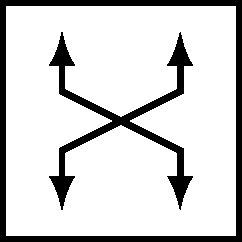
\includegraphics[width=0.9cm,alt={switch}]{../common/fig-switch.pdf}
}
\providecommand{\bigswitch}{%
    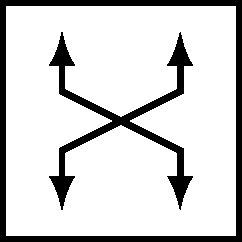
\includegraphics[width=1.4cm,alt={switch}]{../common/fig-switch.pdf}
}
\providecommand{\router}{%
    
\includegraphics[width=0.9cm,alt={router}]{../common/fig-router.pdf}
}



\begin{frame}{exercise}
\myalttext{
\begin{tikzpicture}
\tikzset{
    connect one/.style={draw,very thick,-Latex},
    connect/.style={draw,very thick,Latex-Latex},
    computer/.style={inner sep=0mm,outer sep=0mm,execute at begin node={\computer}},
    switch/.style={inner sep=0mm,outer sep=0mm,execute at begin node={\switch}},
    big switch/.style={inner sep=0mm,outer sep=0mm,execute at begin node={\bigswitch}},
    packet/.style={minimum width=.4cm,minimum height=0.2cm,inner sep=0mm,outer sep=0mm,draw},
    packet lg/.style={minimum width=.6cm,minimum height=0.2cm,inner sep=0mm,outer sep=0mm,draw},
    c1c2/.style={fill=violet!40,draw=black,thin,slidealt=<2>{thick,draw=red}},
}
\node[computer,label={center:A}] (A) at (0, 0) {};
\node[computer,label={center:B}] (B) at (5, -2) {};
\node[computer,label={center:C}] (C) at (10, 0) {};
\node[switch,label={south:S1}] (S1) at (3, 0) {};
\node[switch,label={south:S2}] (S2) at (5, 0) {};
\node[switch,label={south:S3}] (S3) at (7, 0) {};
\draw[connect] (A) -- (S1);
\draw[connect] (S1) -- (S2);
\draw[connect] (B) -- (S2);
\draw[connect] (S2) -- (S3);
\draw[connect] (S3) -- (C);
\end{tikzpicture}
}{A <-> S1 <-> S2 <-> {B, S3 <-> C}}
\begin{itemize}
\item suppose A, B, C all sending to each other (all 6 pairs).
\item where does multiplexing/demultiplexing happen?
\item where are packet drops likely?
\end{itemize}
\end{frame}


\subsection{store and forward}

\begin{frame}\frametitle{buffer usage: fast to slow, store + forward}
\myalttext{
\begin{tikzpicture}
\tikzset{
    axis/.style={draw,thick,-Latex},
    scale mark/.style={draw,thin},
    scale label/.style={font=\small},
    packet/.style={ultra thick,fill=violet!20},
    y=.6cm
}
\begin{scope} % input
    \begin{scope}[shift={(0.1, 0)}]
        \clip (0, 0) rectangle (12.5, 3.2);
        \draw[packet] (0, 0) coordinate (A recv start) rectangle (2, 3) node[midway] {packet A};
        \draw[packet] (2, 0) rectangle (4, 3) node[midway] {packet B};
        \draw[packet] (4, 0) rectangle (6, 3) node[midway] {packet C};
        \draw[packet] (10, 0) rectangle (12, 3) node[midway] {packet D};
    \end{scope}
    \draw[axis] (0, 0) -- ++ (12.5, 0);
    \draw[axis] (0, 0) -- ++ (0, 3.3)
        node[midway,left=.5cm,align=right] { input };
    \draw[scale mark] (0, 3) -- ++ (.25, 0) node[pos=0,left,scale label] {capacity};
\end{scope} 
\begin{scope}[shift={(0, -5)}]% buffer usage
    \begin{scope}
        \clip (0,0) rectangle (12.5, 4);
        \draw[violet, ultra thick] (0, 0) -- (0.1, 0) -- (0.1, 1) -- (2.1, 1) -- (2.1, 2) -- (4.1, 2) -- (4.1, 3)
            -- (5.1, 3) -- (5.1, 2) -- (8.1, 2) -- (8.1, 1) -- (10.1, 1) -- (10.1, 2) -- 
            (11.1, 2) -- (11.1, 1) -- (14, 1);
    \end{scope}
    \draw[axis] (0, 0) -- ++ (12.5, 0);
    \draw[axis] (0, 0) -- ++ (0, 4.3)
    node[midway,left=.5cm,align=right] (usage label) { buffer \\ reserved };
    \node[font=\small,anchor=north,align=center] at (usage label.south) {
        packets
    };
    \draw[scale mark] (0, 1) -- ++ (.25, 0) node[pos=0,left,scale label] {1};
    \draw[scale mark] (0, 2) -- ++ (.25, 0) node[pos=0,left,scale label] {2};
    \draw[scale mark] (0, 3) -- ++ (.25, 0) node[pos=0,left,scale label] {3};
    \draw[scale mark] (0, 4) -- ++ (.25, 0) node[pos=0,left,scale label] {4};
%
\end{scope}
\begin{scope}[shift={(0, -8)}] % output
    \begin{scope}
        \clip (0, 0) rectangle (12.5, 2.2);
        \begin{scope}[shift={(2.1, 0)}]
            \draw[packet] (0, 0) coordinate (A send start) rectangle (3, 2) node[midway] {packet A};
            \draw[packet] (3, 0) rectangle (6, 2) node[midway] {packet B};
            \draw[packet] (6, 0) rectangle (9, 2) node[midway] {packet C};
            \draw[packet] (10, 0) rectangle (13, 2) node[midway] {packet D};
        \end{scope}
    \end{scope}
    \draw[axis] (0, 0) -- ++ (12.5, 0);
    \draw[axis] (0, 0) -- ++ (0, 2.3)
        node[midway,left=.5cm,align=right] { output };
    \draw[scale mark] (0, 2) -- ++ (.25, 0) node[pos=0,left,scale label] {capacity};
\end{scope}
\begin{visibleenv}<2>
    \draw[draw=red,dotted,ultra thick,Latex-Latex] (A send start) -- ++(-2cm, 0);
    \draw[draw=red,dotted,ultra thick] (A send start) -- ++(0cm, 6cm);
    \draw[draw=red,dotted,ultra thick] ([xshift=-2cm]A send start) -- ++(0cm, 6cm);
    \node[draw=red,ultra thick,align=left,fill=white,anchor=west] at  (2.2, -3) {
        \textit{store and forward} \\
        switch stores whole packet in buffer\\
        then sends it out \\
        ~ \\
        our default in this class
    };
\end{visibleenv}
\end{tikzpicture}
}{
*store and forward* switches are illustrated as taking in packets and buffering them
as they received, and only sending packets after they are fully contained in the buffer.
These are the most common type of switches, by far.
}
\end{frame}

\begin{frame}\frametitle{buffer usage: fast to slow, cut-through}
\myalttext{
\begin{tikzpicture}
\tikzset{
    axis/.style={draw,thick,-Latex},
    scale mark/.style={draw,thin},
    scale label/.style={font=\small},
    packet/.style={ultra thick,fill=violet!20},
    y=.6cm
}
\begin{scope} % input
    \begin{scope}[shift={(0.1, 0)}]
        \clip (0, 0) rectangle (12.5, 3.2);
        \draw[packet] (0, 0) coordinate (A recv start) rectangle (2, 3) node[midway] {packet A};
        \draw[packet] (2, 0) rectangle (4, 3) node[midway] {packet B};
        \draw[packet] (4, 0) rectangle (6, 3) node[midway] {packet C};
        \draw[packet] (10, 0) rectangle (12, 3) node[midway] {packet D};
    \end{scope}
    \draw[axis] (0, 0) -- ++ (12.5, 0);
    \draw[axis] (0, 0) -- ++ (0, 3.3)
        node[midway,left=.5cm,align=right] { input };
    \draw[scale mark] (0, 3) -- ++ (.25, 0) node[pos=0,left,scale label] {capacity};
\end{scope} 
\begin{scope}[shift={(0, -5)}]% buffer usage
    \begin{scope}
        \clip (0,0) rectangle (12.5, 4);
        \draw[violet, ultra thick] (0, 0) -- (0.1, 0) -- (0.1, 1) -- (2.1, 1) -- (2.1, 2) -- 
            (3.6, 2) -- (3.6, 1) -- (4.1, 1) -- (4.1, 2) -- (6.6, 2) -- (6.6, 1) --
            (9.6, 1) -- (9.6, 0) -- (10.1, 0) -- (10.1, 1) -- (13.6, 1) -- (13.6, 0);
    \end{scope}
    \draw[axis] (0, 0) -- ++ (12.5, 0);
    \draw[axis] (0, 0) -- ++ (0, 4.3)
    node[midway,left=.5cm,align=right] (usage label) { buffer \\ reserved };
    \node[font=\small,anchor=north,align=center] at (usage label.south) {
        packets
    };
    \draw[scale mark] (0, 1) -- ++ (.25, 0) node[pos=0,left,scale label] {1};
    \draw[scale mark] (0, 2) -- ++ (.25, 0) node[pos=0,left,scale label] {2};
    \draw[scale mark] (0, 3) -- ++ (.25, 0) node[pos=0,left,scale label] {3};
    \draw[scale mark] (0, 4) -- ++ (.25, 0) node[pos=0,left,scale label] {4};
%
\end{scope}
\begin{scope}[shift={(0, -8)}] % output
    \begin{scope}
        \clip (0, 0) rectangle (12.5, 2.2);
        \begin{scope}[shift={(0.6, 0)}]
            \draw[packet] (0, 0) coordinate (A send start) rectangle (3, 2) node[midway] {packet A};
            \draw[packet] (3, 0) rectangle (6, 2) node[midway] {packet B};
            \draw[packet] (6, 0) rectangle (9, 2) node[midway] {packet C};
            \draw[packet] (10, 0) rectangle (13, 2) node[midway] {packet D};
        \end{scope}
    \end{scope}
    \draw[axis] (0, 0) -- ++ (12.5, 0);
    \draw[axis] (0, 0) -- ++ (0, 2.3)
        node[midway,left=.5cm,align=right] { output };
    \draw[scale mark] (0, 2) -- ++ (.25, 0) node[pos=0,left,scale label] {capacity};
\end{scope}
\begin{visibleenv}<1>
    \draw[draw=red,dotted,ultra thick] (A send start) -- ++(-.5cm, 0);
    \draw[draw=red,dotted,ultra thick] (A send start) -- ++(0cm, 6cm);
    \draw[draw=red,dotted,ultra thick] ([xshift=-.5cm]A send start) -- ++(0cm, 6cm);
    \node[draw=red,ultra thick,align=left,fill=white,anchor=west] at  (2.2, -3) {
        \textit{cut-through} forwarding \\
        switch sends packet out as it's being received \\
        ~ \\
        uncommon and much more complex to implement
    };
\end{visibleenv}
\end{tikzpicture}
}{
*cut-through* switches are illustrated as sending packets as they are being received
as long as no other packets are waiting. Though more efficient,
these are uncommon as they are more difficult to implement than
store-and-forward switches (because of, for example, error handling)
}
\end{frame}
% FIXME: multiplexing at end hosts


\subsection{types of channels}

\begin{frame}\frametitle{channel abstractions}
\begin{itemize}
    \item want to avoid custom network for each application
    \item but applications have different needs
    \vspace{.5cm}
    \item $\rightarrow$ multiple application interfaces to networks
    \item common implementation of \myemph{common patterns}
\end{itemize}
\end{frame}

\begin{frame}\frametitle{some abstractions}
    \begin{itemize}
    \item \myemph<2>{stream}
        \begin{itemize}
        \item continuous stream of bytes from one program to another
        \item `connection' from one program to another
        \end{itemize}
    \item datagrams
        \begin{itemize}
        \item send small messages (\textit{datagrams})
        \item each datagram's destination independently set
        \end{itemize}
    \item remote procedure calls
        \begin{itemize}
        \item make function calls that run on remote machine
        \end{itemize}
    \item remote memory access
        \begin{itemize}
        \item read/write bytes of data in remote memory
        \end{itemize}
    \item \ldots
    \end{itemize}
\end{frame}

\begin{frame}\frametitle{focus on streams}
    \begin{itemize}
    \item this class: focus on implementing \textit{streams of bytes}
    \vspace{.5cm}
    \item why?
        \begin{itemize}
        \item most commonly used by applications on the Internet
        \item many common tasks with other abstractions
        \end{itemize}
    \end{itemize}
\end{frame}


\subsubsection{channels and sockets}
\begin{frame}{stream abstraction and sockets}
    \begin{itemize}
    \item BSD \textit{sockets} are most used abstract for using \textit{streams}
    \item server (passive end)
        \begin{itemize}
        \item create socket (\texttt{socket()})
        \item select address (\texttt{bind()})
        \item wait for+get connection (\texttt{listen()}+\texttt{accept()})
        \item read+write on connection(\texttt{read()}+\texttt{recv*()}+\texttt{write()}+\texttt{send*()})
        \end{itemize}
    \item client (active end)
        \begin{itemize}
        \item create socket (\texttt{socket()})
        \item connect to address (\texttt{connect()}
        \item read+write on connection(\texttt{read()}+\texttt{recv*()}+\texttt{write()}+\texttt{send*()})
        \end{itemize}
    \end{itemize}
\end{frame}

\begin{frame}{sockets and other options}
    \begin{itemize}
    \item sockets can also provide \textit{datagram} abstraction
        \begin{itemize}
        \item difference: mode where read/write keeps messages together
        \end{itemize}
    \end{itemize}
\end{frame}

\begin{frame}{socket details later}
    \begin{itemize}
    \item we're doing mostly bottom-up approach
    \item will actually talk in detail about socket interface later in semester
    \end{itemize}
\end{frame}

% FIXME:
    % abstraction provided to application
        % seen sockets
        % datagrams versus streams

\subsubsection{client/server}
\begin{frame}\frametitle{client/server}
    \begin{itemize}
    \item \textit{server} = entity that waits for + responds to \textit{clients}
    \item server:
        \begin{itemize}
        \item always-on
        \item well-known how to contact
        \end{itemize}
    \item client
        \begin{itemize}
        \item sometimes on
        \item only contacted by server responding to it
        \end{itemize}
    \end{itemize}
\end{frame}

\begin{frame}\frametitle{not client/server?}
    \begin{itemize}
    \item not everything fits into client/server neatly
    \vspace{.5cm}
    \item sometimes something is both client and server
    \item sometimes no distinguished entities (``peer-to-peer'')
    \end{itemize}
\end{frame}

\begin{frame}\frametitle{client/server and channels}
    \begin{itemize}
    \item can have channels without client/server model
    \vspace{.5cm}
    \item but the interface sockets provide assume client/server
        \begin{itemize}
        \item (so you have to make something server-like to do peer-to-peer with sockets)
        \end{itemize}
    \end{itemize}
\end{frame}


\subsection{exercise: terms}
\usetikzlibrary{arrows.meta,calc,shapes}
\providecommand{\computer}{%
    
\includegraphics[width=1cm,alt=computer]{../common/Noun_project_216.pdf}
}
\providecommand{\switch}{%
    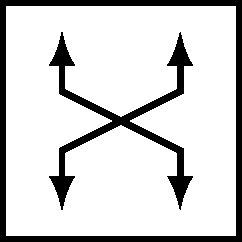
\includegraphics[width=0.9cm,alt=switch]{../common/fig-switch.pdf}
}
\providecommand{\router}{%
    
\includegraphics[width=0.9cm,alt=router]{../common/fig-router.pdf}
}

\begin{frame}[fragile]\frametitle{exercise} % FIXME: text description
\myalttext{
\begin{tikzpicture}
\tikzset{
    computer/.style={inner sep=0mm,outer sep=0mm,execute at begin node={\computer}},
    switch/.style={inner sep=0mm,outer sep=0mm,execute at begin node={\switch}},
    router/.style={inner sep=0mm,outer sep=-1mm,execute at begin node={\router},circle},
    connect/.style={draw,very thick,Latex-Latex},
    connect big/.style={draw,ultra thick,Latex-Latex},
    other/.style={opacity=0.5},
}
\node[computer,label={north:video stream server}] (server) at (0, 0) {};
\node[computer,label={south:user C}] (C) at (6, 0) {};
\node[computer,label={south:user D}] (D) at (6, -2) {};
\node[computer,label={south:user A}] (A) at (-6, 0) {};
\node[computer,label={south:user B}] (B) at (-6, -2) {};
\node[computer,other] (other1) at (-4.3, 0) {};
\node[computer,other] (other2) at (4.5, 0.5) {};
\node[switch] (other3) at (-2,-1) {};
\node[computer,other] (other4) at (-2.7, 0.2) {};
\node[switch] (s1) at (-3, -2) {};
\node[router] (s2) at (0, -2) {};
\node[switch] (s3) at (2, -1) {};
\node[switch] (s4) at (4, -2) {};
\foreach \x/\y in {A/s1,B/s1,s1/s2,server/s2,s2/s3,s3/s4,s4/D,s3/C,s1/other1,s3/other2,s2/other3,other3.west/other4} {
    \draw[connect] (\x) -- (\y);
}
\end{tikzpicture}
}{video stream server <-> circle <-> {square <-> {user C, square <-> used D}, square <-> unlabeled computer, square <-> {user A, user B}}}
    \begin{itemize}
    \item if each of users A--D are receiving (potentially different) video 
    and audio from the video streaming server, then\ldots
        \begin{itemize}
        \item how many flows?
        \item how many nodes are involved?
        \item how many switches/routers?
        \end{itemize}
    \end{itemize}
\end{frame}



\section{standardization}
\begin{frame}{IETF}
    \begin{itemize}
    \item IETF = Internet Engineering Task Force
        \begin{itemize}
        \item part of non-profit called \textit{Internet Society}
        \end{itemize}
    \item most common internet protocols standardized by IETF
    \item most IETF documents called \myemph{RFCs}
        \begin{itemize}
        \item requests for comment
        \item have unique number
        \end{itemize}
    \item \url{https://rfc-editor.org}
    \end{itemize}
\end{frame}

\begin{frame}{other standard orgs}
    \begin{itemize}
        \item Bluetooth Special Interest Group
        \item IEEE (Institute of Electrical and Electronics Engineers)
            \begin{itemize}
            \item Wifi, Ethernet, \ldots
            \end{itemize}
        \item 3GPP (3rd Generation Partnership Project)
            \begin{itemize}
            \item cellular phone networks
            \end{itemize}
        \item SCTE (Society of Cable Televsion Engineers)
        \item ITU (International Telecommunication Union)
        \item ISO (International Organization for Standardization)
    \end{itemize}
\end{frame}


\section{building with layers}

\subsection{separation of responsibility}

\begin{frame}\frametitle{some challenges for streams}
    \begin{itemize}
    \item separating data into pieces network can handle
    \item \myemph<4>{putting pieces back together}
    \item \myemph<4,5>{getting network to send piece to correct remote network}
    \item \myemph<3,5>{getting network to send piece to correct machine}
    \item \myemph<4>{getting machine to send data to correct program}
    \item \myemph<3,5>{getting pieces into format wires/radio/fiber/etc. can handle}
    \item handling transmission errors
    \end{itemize}
\begin{tikzpicture}[overlay,remember picture]
\begin{visibleenv}<2>
    \node[draw=red,fill=white,ultra thick] at (current page.center) {
        lots of work! don't want to implement all at once!
    };
\end{visibleenv}
\begin{visibleenv}<3>
    \node[draw=red,fill=white,ultra thick] at ([yshift=2cm]current page.center) {
        some parts need to be different for different local networks
    };
\end{visibleenv}
\begin{visibleenv}<4>
    \node[draw=red,fill=white,ultra thick] at ([yshift=3cm]current page.center) {
        some parts should not concern local network implementors
    };
\end{visibleenv}
\begin{visibleenv}<5>
    \node[draw=red,fill=white,ultra thick] at ([yshift=3cm]current page.center) {
        some parts should be same for different abstraction
    };
\end{visibleenv}
\end{tikzpicture}
\end{frame}

\begin{frame}\frametitle{layered model}
    \begin{itemize}
    \item networking implemented in `layers'
    \item upper layers implemented by making calls to lower layers
    \vspace{.5cm}
    \item example: network implements `send data to (remote) machine' function (``network layer'')
    \item stream implementation calls this to implement `send stream to remote application'
    \end{itemize}
\end{frame}



\subsection{OSI/Internet model}

\usetikzlibrary{calc}

\begin{frame}{OSI model}
\begin{tikzpicture}
\node (osi) at (0,0) {
    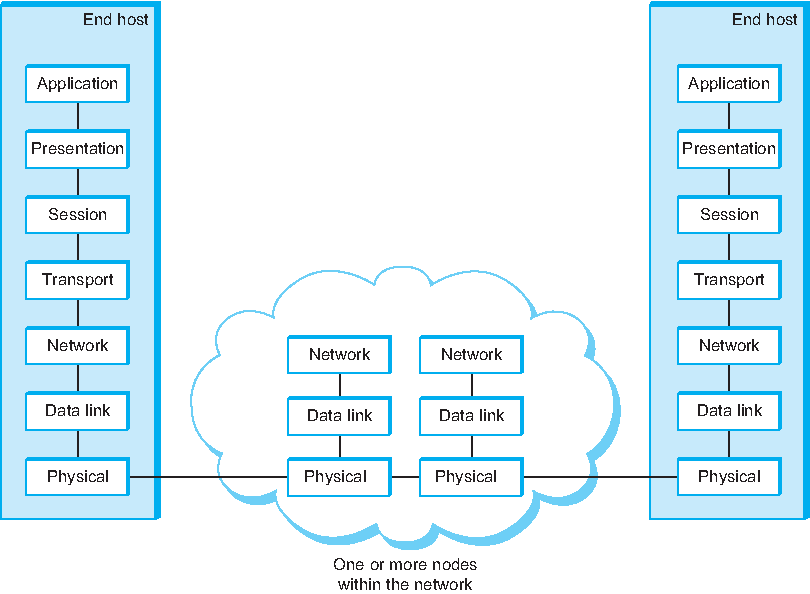
\includegraphics[height=0.75\textheight]{../intro/systemsapproach-1-fig-13.pdf}
};
\coordinate[overlay] (explain loc) at ([yshift=1cm,xshift=0cm]osi.north east);
\tikzset{
    explain box/.style={font=\small,alt=<2>{draw=red}{draw=black},very thick,align=left,at={(explain loc)}, anchor=north west},
    alt explain box/.style={draw=red,ultra thick,anchor=north east,align=left,at={([yshift=-1cm]explain loc)},fill=white},
}
\begin{visibleenv}<2->
\node[overlay,explain box] {
    (7) \myemph<3>{application}: \\ \hspace{.5cm}what requests/etc. \\
    (6) \myemph<3>{presentation}: \\ \hspace{.5cm}data format \\
    (5) \myemph<3>{session}: \\ \hspace{.5cm}manage group of streams \\
    (4) transport: \\ \hspace{.5cm}streams of data \\
    (3) network: \\ \hspace{.5cm}message to correct network \\
    (2) data link: \\ \hspace{.5cm}message $\rightarrow$ bits \\
    \hspace{.5cm}message to correct machine \\
    (1) physical: \\ \hspace{.5cm}send bits/\ldots 
};
\end{visibleenv}
\begin{visibleenv}<3>
\node[overlay,alt explain box] {
    current Internet \\
    usually* layers 5--7 merged together
};
\end{visibleenv}
\end{tikzpicture}
\imagecredit{Figure 13 of Chapter 1 of Computer Networks: A Systems Approach (6th ed) (Peterson and Davie)}
\end{frame}

\begin{frame}<0>{OSI model (text)}
\begin{tabular}{lll} \hline
7 & \myemph<2>{application} & what requests/etc. \\ \hline 
6 & \myemph<2>{presentation} & format of data \\ \hline 
5 & \myemph<2>{session} & coordinate multiple streams \\ \hline
4 & transport & streams of data \\ \hline
3 & network & message to correct network \\ \hline
2 & data link & message to correct machine \\ 
~ & ~ & message into bits/symbols \\
1 & physical & transmit bits/symbols on medium \\
\end{tabular}
\begin{itemize}
\item<2-> \myemph<2>{internet: usually combines layers 7/6/5}
\end{itemize}
\end{frame}

\begin{frame}{OSI model}
    \begin{itemize}
    \item standardized by ISO (International Standards Organization) and ITU (International Telecommunications Union)
    \item full set of protocols\ldots
        \begin{itemize}
        \item file transfer, message sending, directory lookups \ldots
        \end{itemize}
    \item that were often implemented and sometimes used\ldots
    \item but mostly lost out to IETF-standardized Internet protocols
        \begin{itemize}
        \item Internet Engineering Task Force
        \end{itemize}
    \end{itemize}
\end{frame}

\begin{frame}{OSI influence (1)}
    \begin{itemize}
    \item term `layer 7', `layer 4', `layer 3', etc. almost always refer to OSI model
    \item \ldots even though most of Internet does not follow it
        \begin{itemize}
        \item early Internet protocols predate OSI
        \end{itemize}
    \end{itemize}
\end{frame}

\begin{frame}{OSI influence (2)}
    \begin{itemize}
    \item are a lot of Internet protocols influenced by OSI protocols
    \vspace{.5cm}
    \item OSI's DAP (directory access protocol) 
        \begin{itemize}
        \item adapted into IETF's LDAP (lightweight directory access protocol)
        \end{itemize}
    \item OSI presentation layer ASN.1 used in\ldots
        \begin{itemize}
        \item telephony (between telephone companies)
        \item inter-bank messaging
        \item lots of cryptography-related protocols
        \item \ldots
        \end{itemize}
    \item OSI's routing protocol IS-IS still common in large Internet-connected networks
        \begin{itemize}
        \item (adapted to work alongside IETF protocols)
        \end{itemize}
    \end{itemize}
\end{frame}

\begin{frame}{Internet layers}
\small
\begin{tabular}{|l|l|l|p{6cm}|} 
OSI layer & name & examples & purpose \\ \hline
7 & application & HTTP, SSH, & {application-defined meanings}\\
~ & ~ & SMTP, DNS, \ldots & ~ \\ \hline
4 & {transport} & TCP, UDP, \ldots & {reach correct program,\linebreak \myemph<2>{reliablity/streams}} \\ \hline
3 & {network} & IPv4, IPv6, \ldots & {reach correct machine}\linebreak(across networks) \\ \hline
2 & {link} & Ethernet, Wi-Fi, \ldots & {coordinate shared wire/radio}\\ \hline
1 & physical & \ldots & encode bits for wire/radio \\ \hline
\end{tabular}
\end{frame}

\begin{frame}{Internet protocols and layers (non-exhaustive)}
\begin{tikzpicture}
\node[anchor=north west] (int) at (0,0) {
    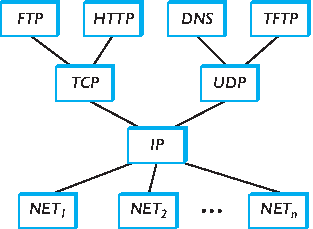
\includegraphics[height=0.75\textheight]{../intro/systemsapproach-1-fig-14.pdf}
};
%\draw[help lines] (0, 0) grid (14, -8);
%\draw[step=2,draw,thick,red] (0, 0) grid (14, -8);
\tikzset{
    layer hi/.style={draw=red,ultra thick},
    layer label/.style={anchor=west},
}
\draw[layer hi] (0, 0) rectangle (9, -1.3);
\node[layer label] at (9.1, -0.65) { application {\it\small OSI layer 7} };
\draw[layer hi] (1.5, -1.8) rectangle (7.5, -3.2);
\node[layer label] at (8.6, -2.5) { transport {\it\small OSI layer 4} };
\draw[layer hi,alt=<2>{fill=red,fill opacity=0.1}] (3.5, -3.6) rectangle (5.6, -4.85);
\node[layer label] at (5.8, -4.2) (net label) { network {\it\small OSI layer 3} };
\draw[layer hi] (0.5, -5.5) rectangle (9, -6.6);
\node[layer label] at (9.1, -6) { data link {\it\small OSI layer 2} };
\begin{visibleenv}<2>
    \node[anchor=west,red,font=\large] at (net label.east) {``narrow waist''};
\end{visibleenv}
\end{tikzpicture}
\imagecredit{Figure 14 of Chapter 1 of Computer Networks: A Systems Approach (6th ed) (Peterson and Davie)}
\end{frame}



\subsection{layers are fuzzy}


\begin{frame}{fuzzy layers (1)}
    \begin{itemize}
    \item ICMP (Internet Control Message Protocol)\ldots
    \item {implemented using a network layer}\ldots
        \begin{itemize}
        \item so seems like a transport layer protocol?
        \end{itemize}
    \item<2-> used to send errors/control messages about routing\ldots
        \begin{itemize}
        \item routing is the network layer's job
        \item so ICMP is part of network layer?
        \end{itemize}
    \vspace{.5cm}
    \item<3-> I think saying network layer is probably better\ldots
    \item<3-> but we're not going to be picky about it
    \end{itemize}
\end{frame}

\begin{frame}{fuzzy layers (2)}
    \begin{itemize}
    \item TLS (Transport Control Protocol)\ldots
    \item implemented on top of TCP\ldots
        \begin{itemize}
        \item so seems like a application layer protocol?
        \end{itemize}
    \item<2-> used to send other application layer protocols
        \begin{itemize}
        \item so maybe a transport layer?
        \item or presentation layer?
        \end{itemize}
    \vspace{.5cm}
    \item<2-> I'll call it an application layer\ldots
    \end{itemize}
\end{frame}

\begin{frame}{`extra' layers}
    \begin{itemize}
    \item layer terminology doesn't always work cleanly
        \begin{itemize}
        \item often ``extra'' layers in practice
        \end{itemize}
    \item e.g. HTTPS:
        \begin{itemize}
        \item HTTP (app layer) on TLS (another app layer) on TCP (network) on \ldots
        \end{itemize}
    \item e.g. \myemph<2>{DNS over HTTPS}:
        \begin{itemize}
        \item DNS (app layer) on HTTP on on TLS on TCP on \ldots
        \end{itemize}
    \item e.g. SFTP:
        \begin{itemize}
        \item SFTP (app layer??) on SSH (another app layer) on TCP on \ldots
        \end{itemize}
    \item e.g. HTTP over OpenVPN:
        \begin{itemize}
        \item HTTP on TCP on IP on OpenVPN on UDP on different IP on \ldots
        \end{itemize}
    \end{itemize}
\end{frame}

\begin{frame}{protocols usually over HTTP}
    \begin{itemize}
    \item SOAP (Simple Object Access Protocol) --- messaging/remote procedure calls
    \item gRPC (originally form Google) --- remote procedure calls
    \item HLS (HTTP Live Streaming) --- video streaming
    \item DASH (Dynamic Adaptive Streaming over HTTP) --- video streaming
    \item \ldots
    \end{itemize}
\end{frame}



\section{interlude: wireshark preview}

% FIXME:
\begin{frame}\frametitle{packet capture tools}
    \begin{itemize}
    \item packet capture = log of everything sent/received on some link(s)
    \item wireshark is popular tool for making, analyzing packet captures
    \vspace{.5cm}
    \item will be showing screenshots from that
    \vspace{.5cm}
    \item you can download these packet captures, follow along in wireshark
    \end{itemize}
\end{frame}

% FIXME: HTTPS

\subsection{some examples in wireshark}
\usetikzlibrary{arrows.meta,decorations.pathreplacing}
\begin{frame}[fragile]{}
\begin{tikzpicture}
\tikzset{
    overlay box/.style={fill=white,fill opacity=0.9}
}
\node[overlay,anchor=north west,inner sep=0mm] (base) at (0, 0) {
    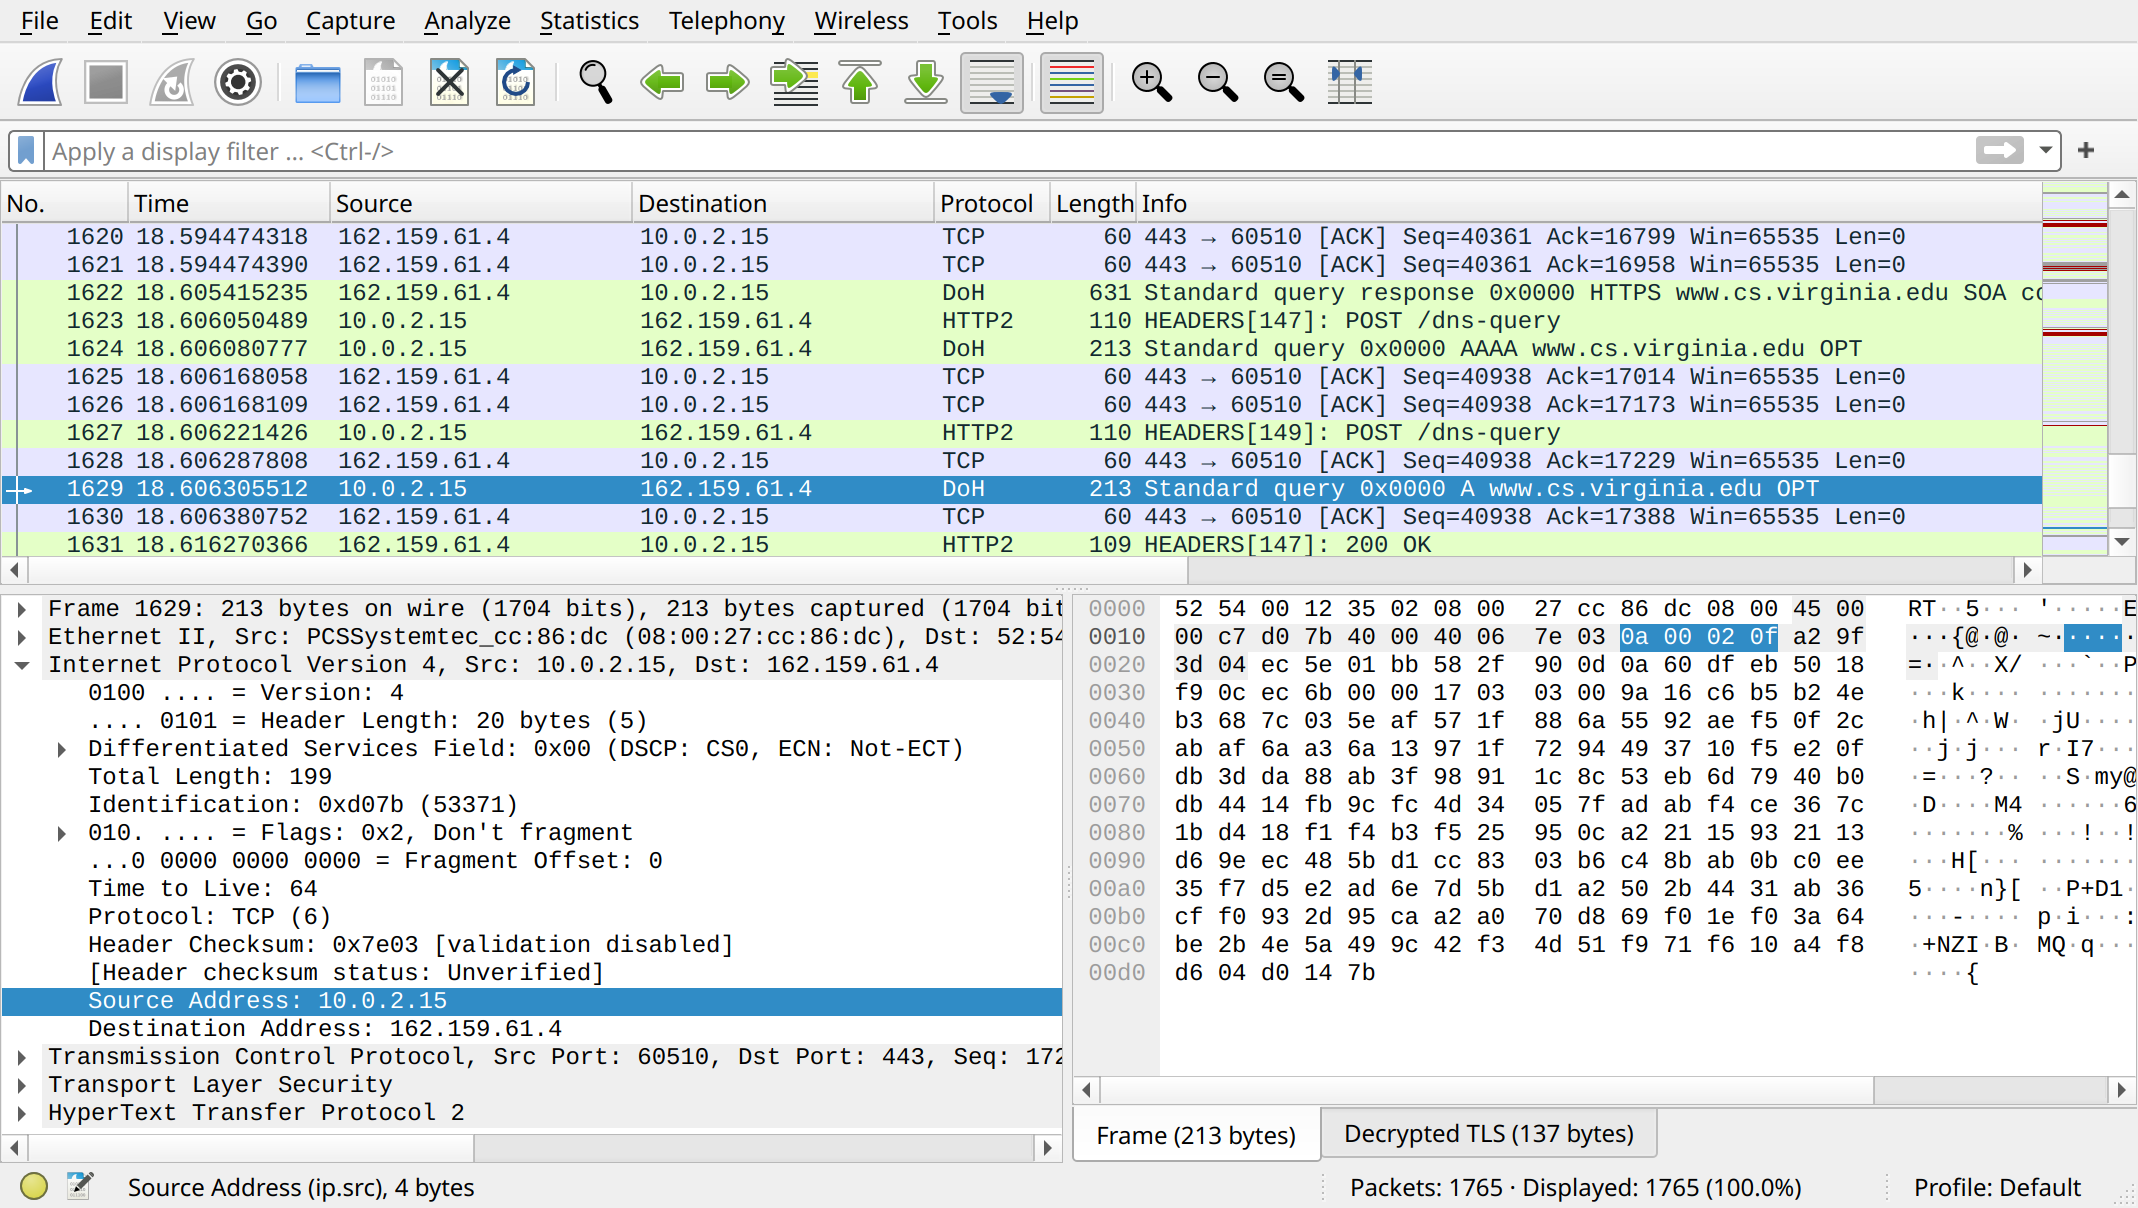
\includegraphics[width=\textwidth]{../intro/wireshark-example1.png}
};
\begin{visibleenv}<1>
    \node[text=red,overlay box] at (7.5, -2) {wireshark window};
\end{visibleenv}
\path (0, 0) rectangle (14.5, -7); % for bounding box
%\draw[overlay,help lines] (0, 0) grid (14, -8);
\begin{visibleenv}<3>
    \path[draw,red,very thick] (0, -1.2) rectangle (14.5, -4)
        node[midway,overlay box] { packet list };
    \path[draw,red,very thick] (0, -4) rectangle (7.25, -7.9)
        node[midway,overlay box] { packet details };
    \path[draw,red,very thick] (7.25, -4) rectangle (14.5, -7.9)
        node[midway,overlay box] { packet bytes };
\end{visibleenv}
\begin{visibleenv}<4>
    \path[draw,red,very thick] (0, -6.7) rectangle (7.2, -6.9);
    \path[draw,red,very thick] (10.93, -4.2) rectangle (12.1, -4.4);
    \path[draw,red,ultra thick] (7.2, -6.8) -- (10.93, -4.3)
        node[midway,above left,overlay box,align=left] {
            hilite in details \\
            shows corresponding bytes
        }
        node[midway,below right,overlay box,font=\fontsize{10}{11}\selectfont,text=black,align=left] {
            this case: \\
            \texttt{10} = \texttt{0x0a} \\
            \texttt{0} = \texttt{0x00} \\
            \texttt{2} = \texttt{0x02} \\
            \texttt{15} = \texttt{0x0f}
        };
\end{visibleenv}
\begin{visibleenv}<5>
    \path[draw,red,very thick] (6.3, -1.2) rectangle (7.15, -4);
    \node[overlay box,anchor=west] at (7.15, -3) (protocol) {`protocol'};
    \node[overlay box,font=\small,anchor=north west] at (protocol.south west) {
        the highest-layer protocol decoded
    };
\end{visibleenv}
\begin{visibleenv}<6-7>
    \begin{scope}
        \begin{pgfinterruptboundingbox}
    \tikzset{invclip/.style={clip,insert path={{[reset cm]
          (-16383.99999pt,-16383.99999pt) rectangle (16383.99999pt,16383.99999pt)
      }}}}
        \path[invclip] (6.3, -3.2) rectangle (7.15, -3.4);
        \end{pgfinterruptboundingbox}

        \fill[overlay,white,fill opacity=0.8] (0, 0) rectangle (14.5, -1.2);
        \fill[white,fill opacity=0.8] (0, -1.2) rectangle (14.5, -4);
        \fill[white,fill opacity=0.8] (7.25, -4) rectangle (14.5, -7.9);
    \end{scope}
    \path[draw,red,very thick] (0, -4) rectangle (7.25, -7.9);
    \tikzset{
        protomark/.style={Latex-,blue,thick},
        protomark brace/.style={blue,thick,decorate,decoration={brace}},
        protomark label/.style={blue,fill=white,fill opacity=0.9},
    }
    \draw[protomark] (7.25, -4.3) -- ++(1, 0) node[right,protomark label] {ethernet};
    \draw[protomark brace] (7.3, -4.5) -- (7.3, -7.1);
        \draw[protomark] (7.4, -5.8) -- ++ (0.75, .6) node[right, protomark label] {
                IPv4 (internet protocol version 4)
        };
    \draw[protomark] (7.25, -7.2) -- ++(1, 1) node[right,protomark label] {
        TCP ({\fontsize{10}{11}\selectfont transmission control protocol})
    };
    \draw[protomark] (7.25, -7.325) -- ++(1, .5) node[right,protomark label] {
        TLS ({\fontsize{10}{11}\selectfont transport layer security})
    };
    \draw[protomark] (7.25, -7.45) -- ++(1, -.2) node[right,protomark label] {
        HTTP/2 ({\fontsize{10}{11}\selectfont hypertext transfer protocol 2})
    };
\end{visibleenv}
\begin{visibleenv}<7>
    \draw[red, very thick] (6.3, -3.2) rectangle (7.15, -3.4);
    \draw[red,Latex-,very thick] (7.15, -3.3) -- ++(1, 0) node[right,align=left,overlay box] {
        DoH is not \\one of these!
    };
\end{visibleenv}
\end{tikzpicture}
\end{frame}

\begin{frame}{}
\begin{tikzpicture}
\tikzset{
    overlay box/.style={fill=white,fill opacity=0.9}
}
\node[overlay,anchor=north west,inner sep=0mm] (base) at (0, 0) {
    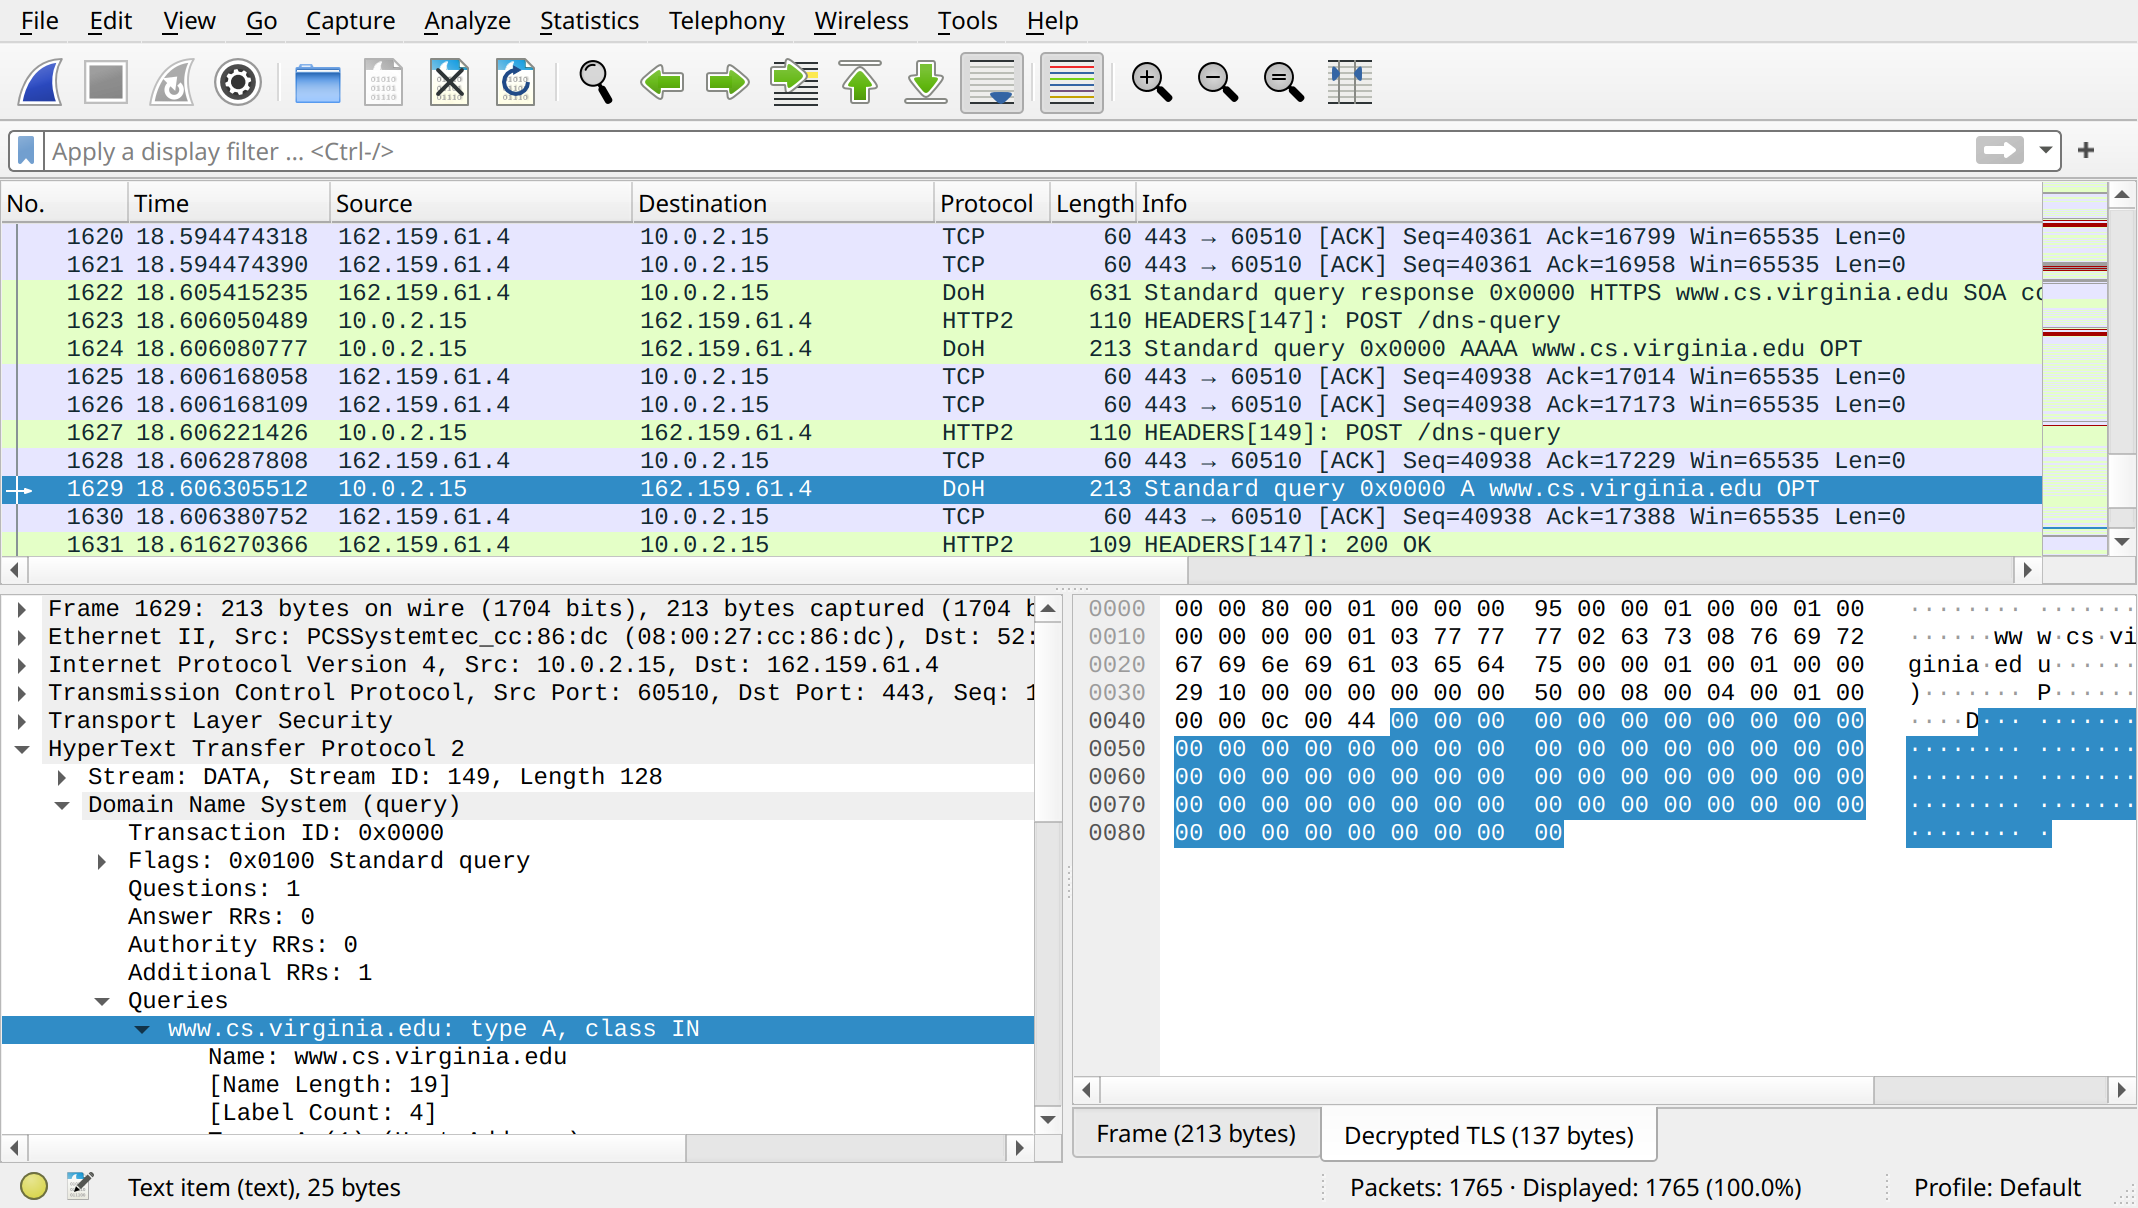
\includegraphics[width=\textwidth]{../intro/wireshark-doh-zoom.png}
};
\path (0, 0) rectangle (14.5, -7); % for bounding box
%\draw[overlay,help lines] (0, 0) grid (14, -8);
    \begin{scope}
        \begin{pgfinterruptboundingbox}
    \tikzset{invclip/.style={clip,insert path={{[reset cm]
          (-16383.99999pt,-16383.99999pt) rectangle (16383.99999pt,16383.99999pt)
      }}}}
        \path[invclip] (6.3, -3.2) rectangle (7.15, -3.4);
        \end{pgfinterruptboundingbox}

        \fill[overlay,white,fill opacity=0.8] (0, 0) rectangle (14.5, -1.2);
        \fill[white,fill opacity=0.8] (0, -1.2) rectangle (14.5, -4);
        \fill[white,fill opacity=0.8] (7.25, -4) rectangle (14.5, -7.9);
    \end{scope}
    \path[draw,red,very thick] (0, -4) rectangle (7.25, -7.9);
    \tikzset{
        protomark/.style={Latex-,blue,thick},
        protomark alt/.style={Latex-,violet,thick,dotted},
        protomark brace/.style={blue,thick,decorate,decoration={brace}},
        protomark brace alt/.style={violet,thick,decorate,decoration={brace}},
        protomark label/.style={blue,fill=white,fill opacity=0.9},
    }
    \draw[protomark] (7.25, -4.3) -- ++(1, .2) node[right,protomark label] {ethernet};
    \draw[protomark] (7.25, -4.5) -- ++ (1, -.2) node[right, protomark label] {
                IPv4 (internet protocol version 4)
        };
    \draw[protomark] (7.25, -4.6) -- ++(1, -.6) node[right,protomark label] {
        TCP ({\fontsize{10}{11}\selectfont transmission control protocol})
    };
    \draw[protomark] (7.25, -4.8) -- ++(1, -1) node[right,protomark label] {
        TLS ({\fontsize{10}{11}\selectfont transport layer security})
    };
    \draw[protomark brace] (7.3, -5) -- (7.3, -7.9);
        \draw[protomark] (7.4, -6.5) -- ++ (0.75, 0) node[right, protomark label] {
            HTTP/2 ({\fontsize{10}{11}\selectfont hypertext transfer protocol 2})
        };
    \draw[protomark brace alt] (7.5, -5.5) -- (7.5, -7.9);
        \draw[protomark alt] (7.6, -6.85) -- ++ (0.75, -.5) node[right, protomark label] {
            DNS (domain name system)
        };
    \draw[red, very thick] (6.3, -3.2) rectangle (7.15, -3.4);
    \draw[red,Latex-,very thick] (7.15, -3.3) -- ++(1, 0) node[right,align=left,overlay box] {
        DoH = DNS over HTTPS
    };
\end{tikzpicture}
\end{frame}

\begin{frame}[fragile]{}
\providecommand{\doHilite}[6]{
    %\doHilite{Y offset start protocol list}{Y offset end protocol list}
    %         {X offset corner data}{Y offset corner data}
    %         {X offset other corner data}{Y offset other corner data}
    \path[draw,red,very thick] (0, -3.95 - #1 * 0.206) rectangle (7.25, -3.95 - #2 * 0.206);
    \path[draw,red,very thick] (7.95 + #3, -4.2059 - #4 * 0.2059) -- (7.95 + #3, -3.95 - #4 * 0.2059)
            -- (12.8, -3.95 - #4 * 0.2059)
            |- (7.95 + #5, -4 - #6 * 0.2059) 
            |- (7.95, -4 - #6 * 0.2059 - .2059) |- cycle;
}
\providecommand{\doHiliteOneDataLine}[6]{
    %\doHilite{Y offset start protocol list}{Y offset end protocol list}
    %         {X offset corner data}{Y offset corner data}
    %         {X offset other corner data}{Y offset other corner data}

    \path[draw,red,very thick] (0, -3.95 - #1 * 0.207) rectangle (7.25, -4 - #2 * 0.207);
    \path[draw,red,very thick] (7.95 + #3, -4.207 - #4 * 0.207) -- (7.95 + #3, -4 - #4 * 0.207)
            %-- (12.8, -4 - #4 * 0.207)
            |- (7.95 + #5, -4 - #6 * 0.207) 
            |- (7.95, -4 - #6 * 0.207 - .207) |- cycle;
}
\begin{tikzpicture}
\tikzset{
    overlay box/.style={fill=white,fill opacity=0.9},
}
\node[overlay,anchor=north west,inner sep=0mm] (base) at (0, 0) {%
\only<1-2>{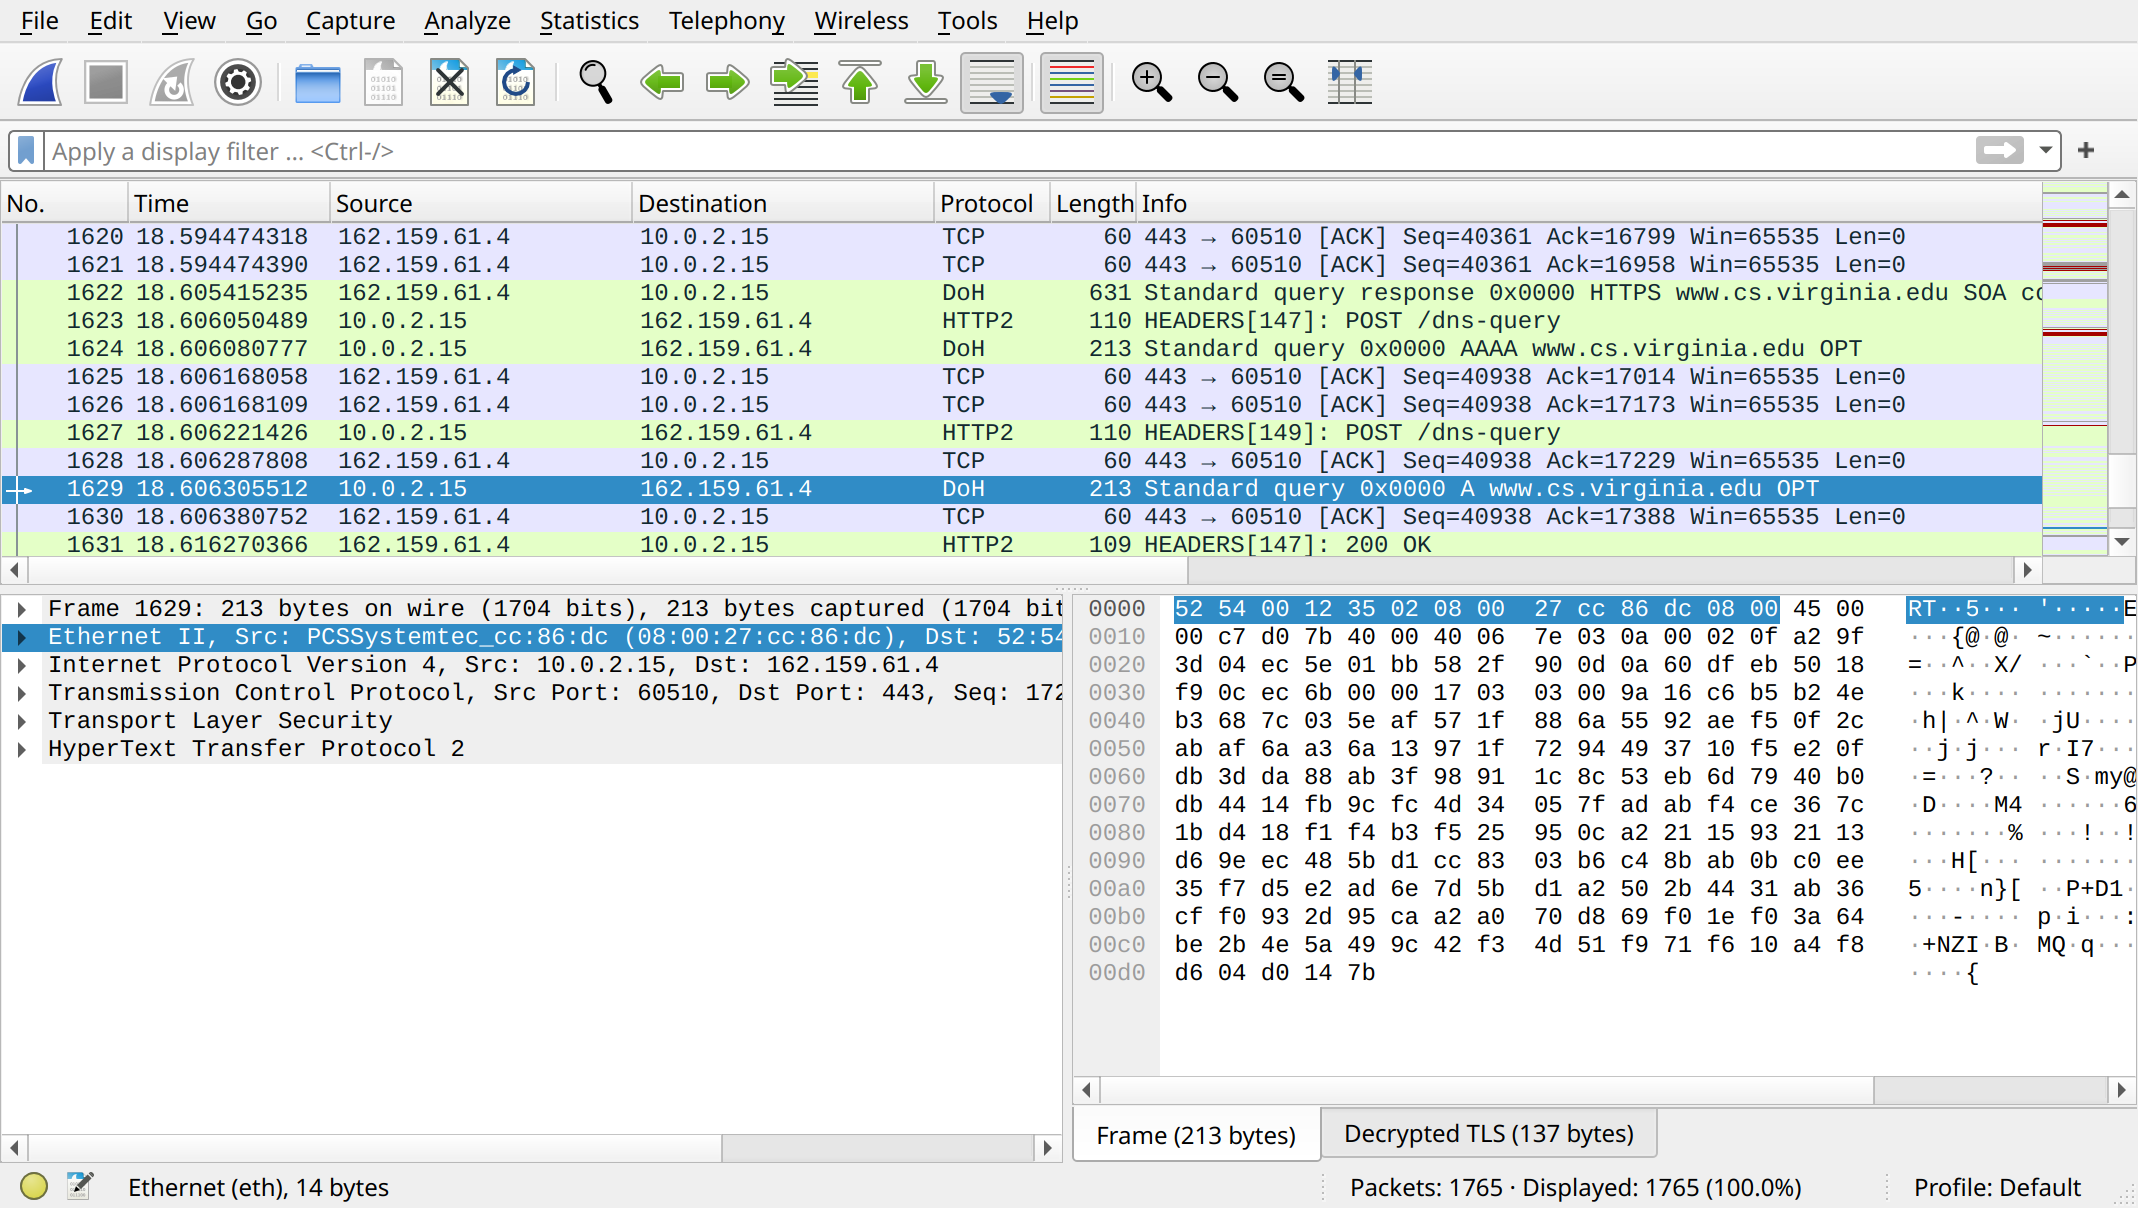
\includegraphics[width=\textwidth]{../intro/wireshark-hi-ethernet.png}}%
\only<3-4>{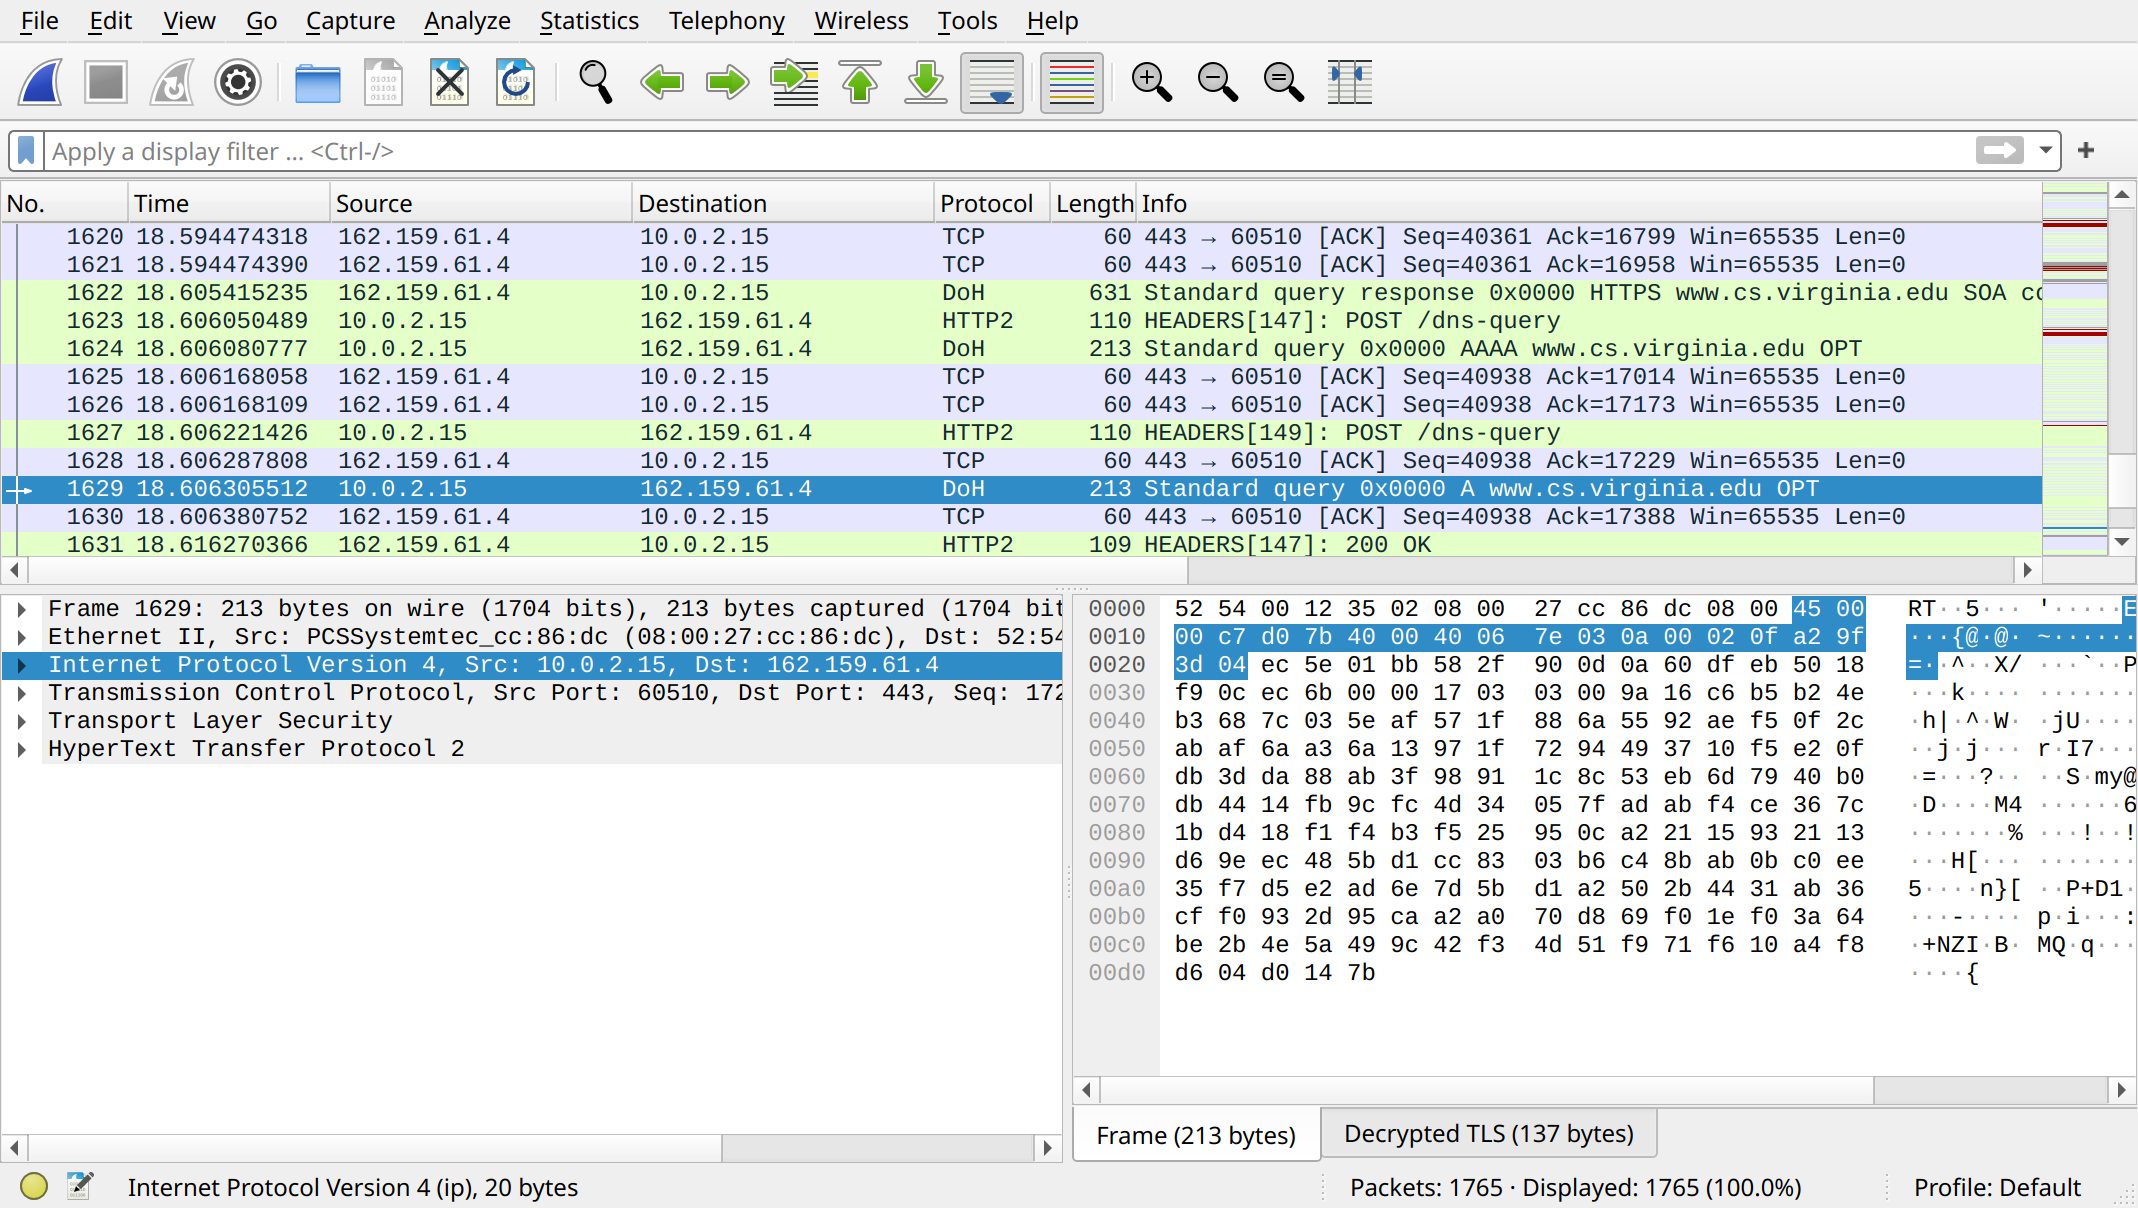
\includegraphics[width=\textwidth]{../intro/wireshark-hi-ipv4.png}}%
\only<5-6>{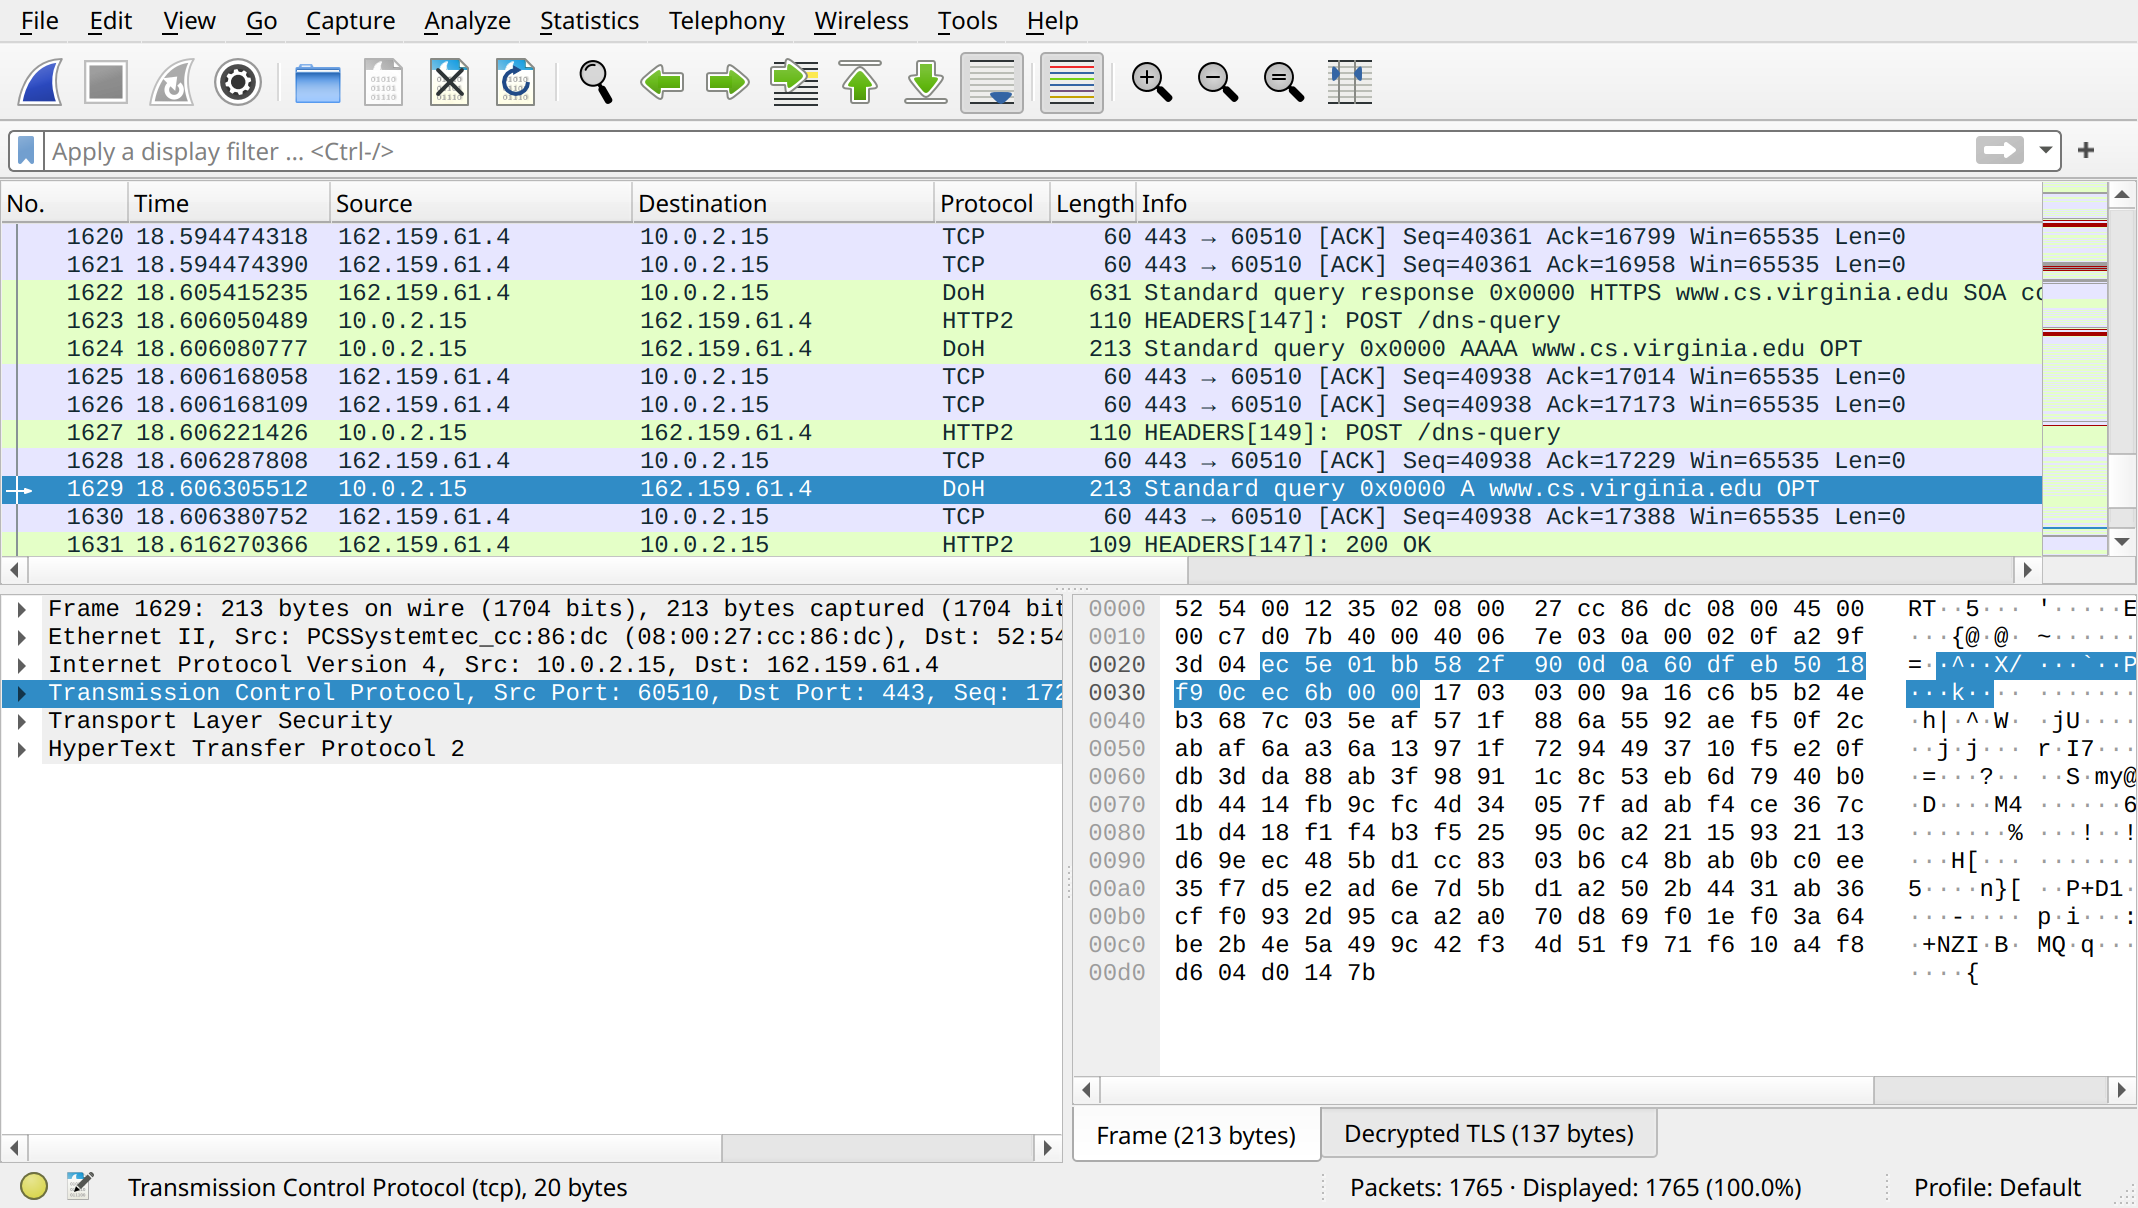
\includegraphics[width=\textwidth]{../intro/wireshark-hi-tcp.png}}%
\only<7-8>{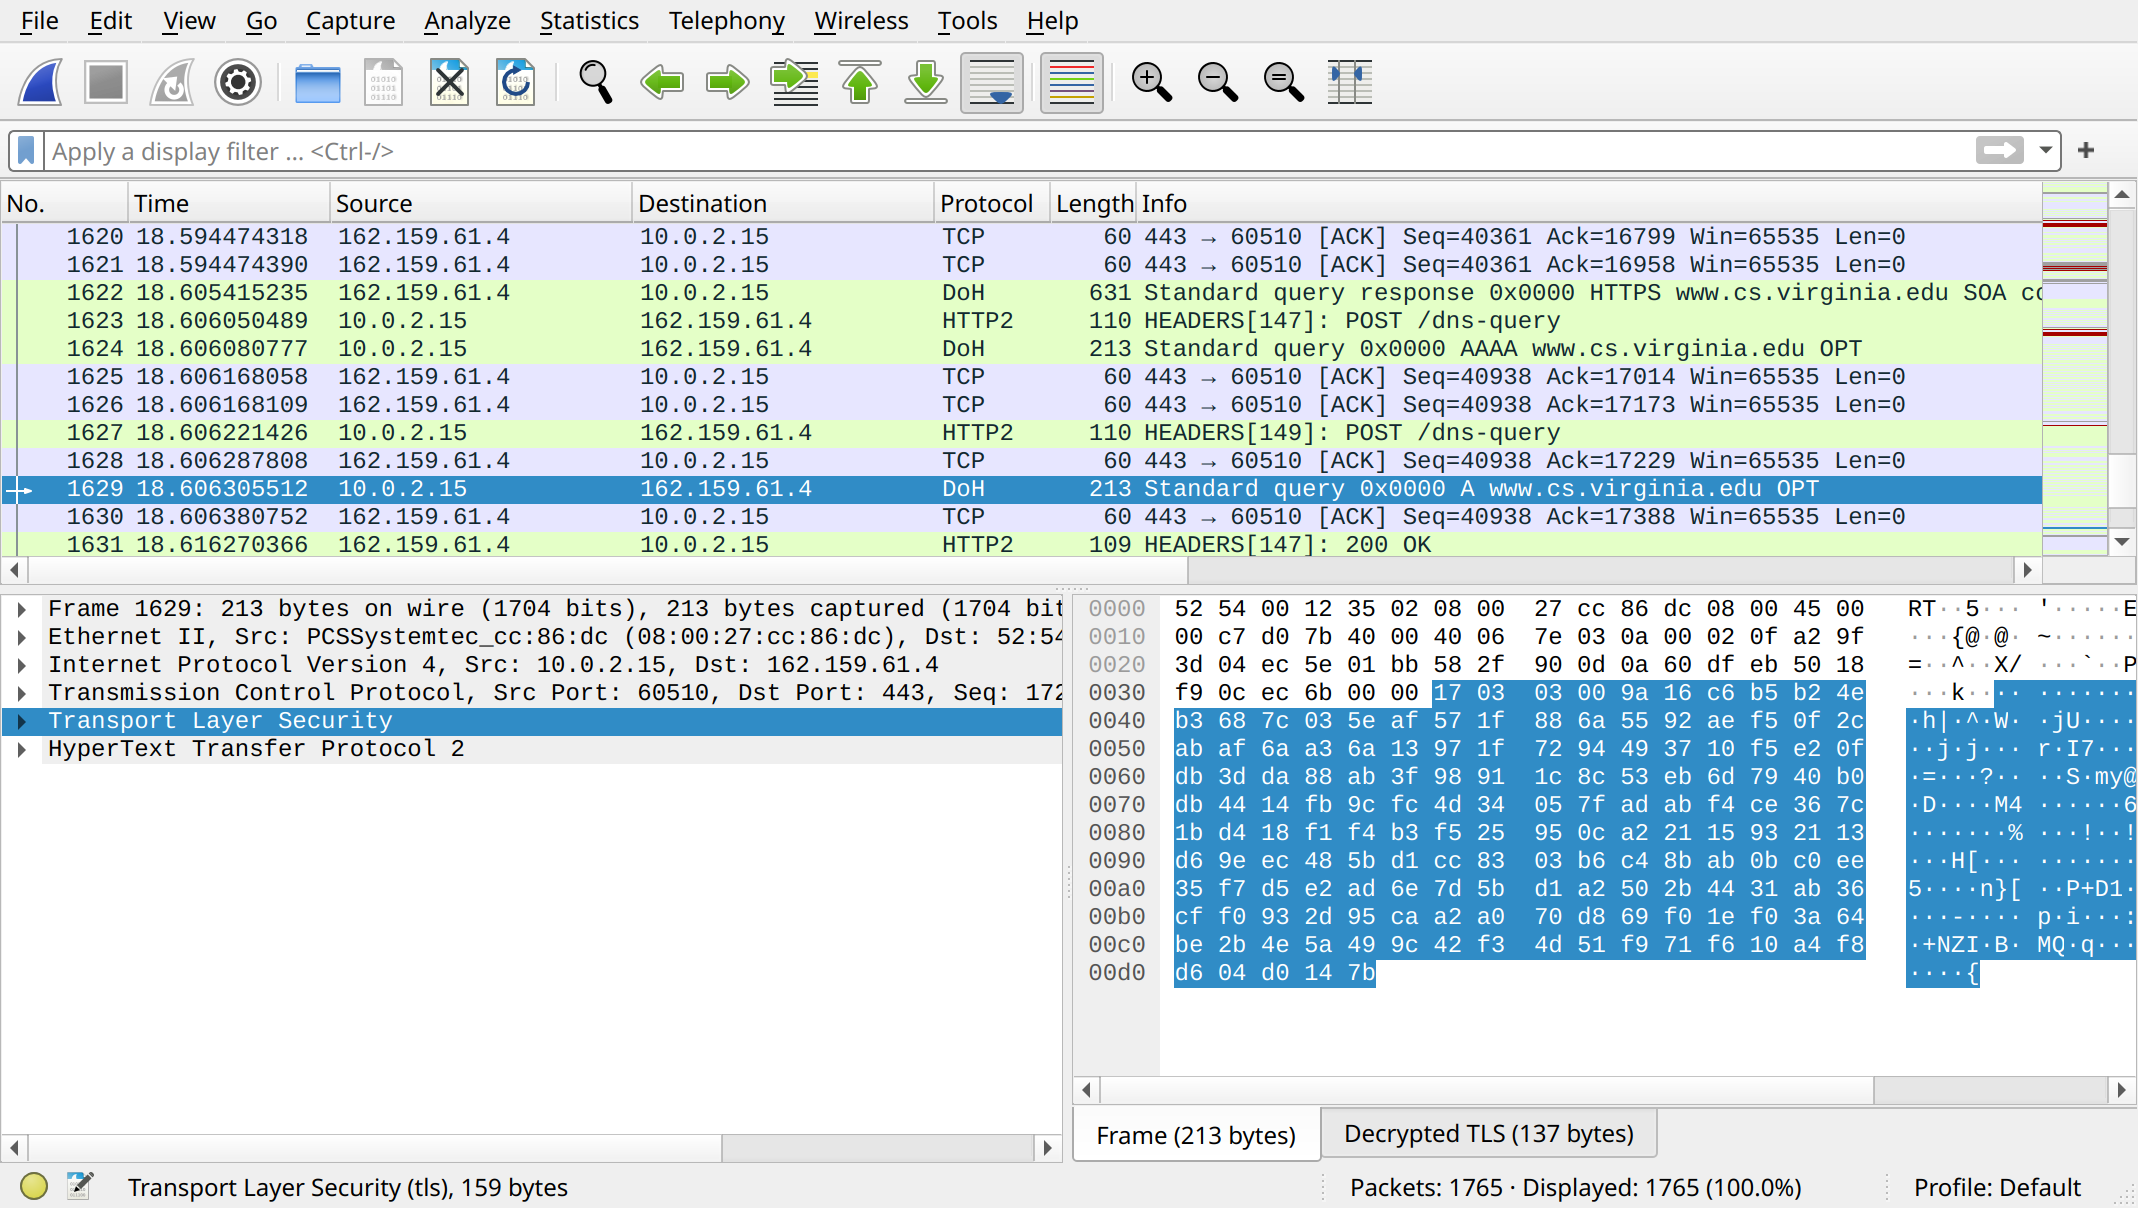
\includegraphics[width=\textwidth]{../intro/wireshark-hi-tls.png}}%
\only<9-11>{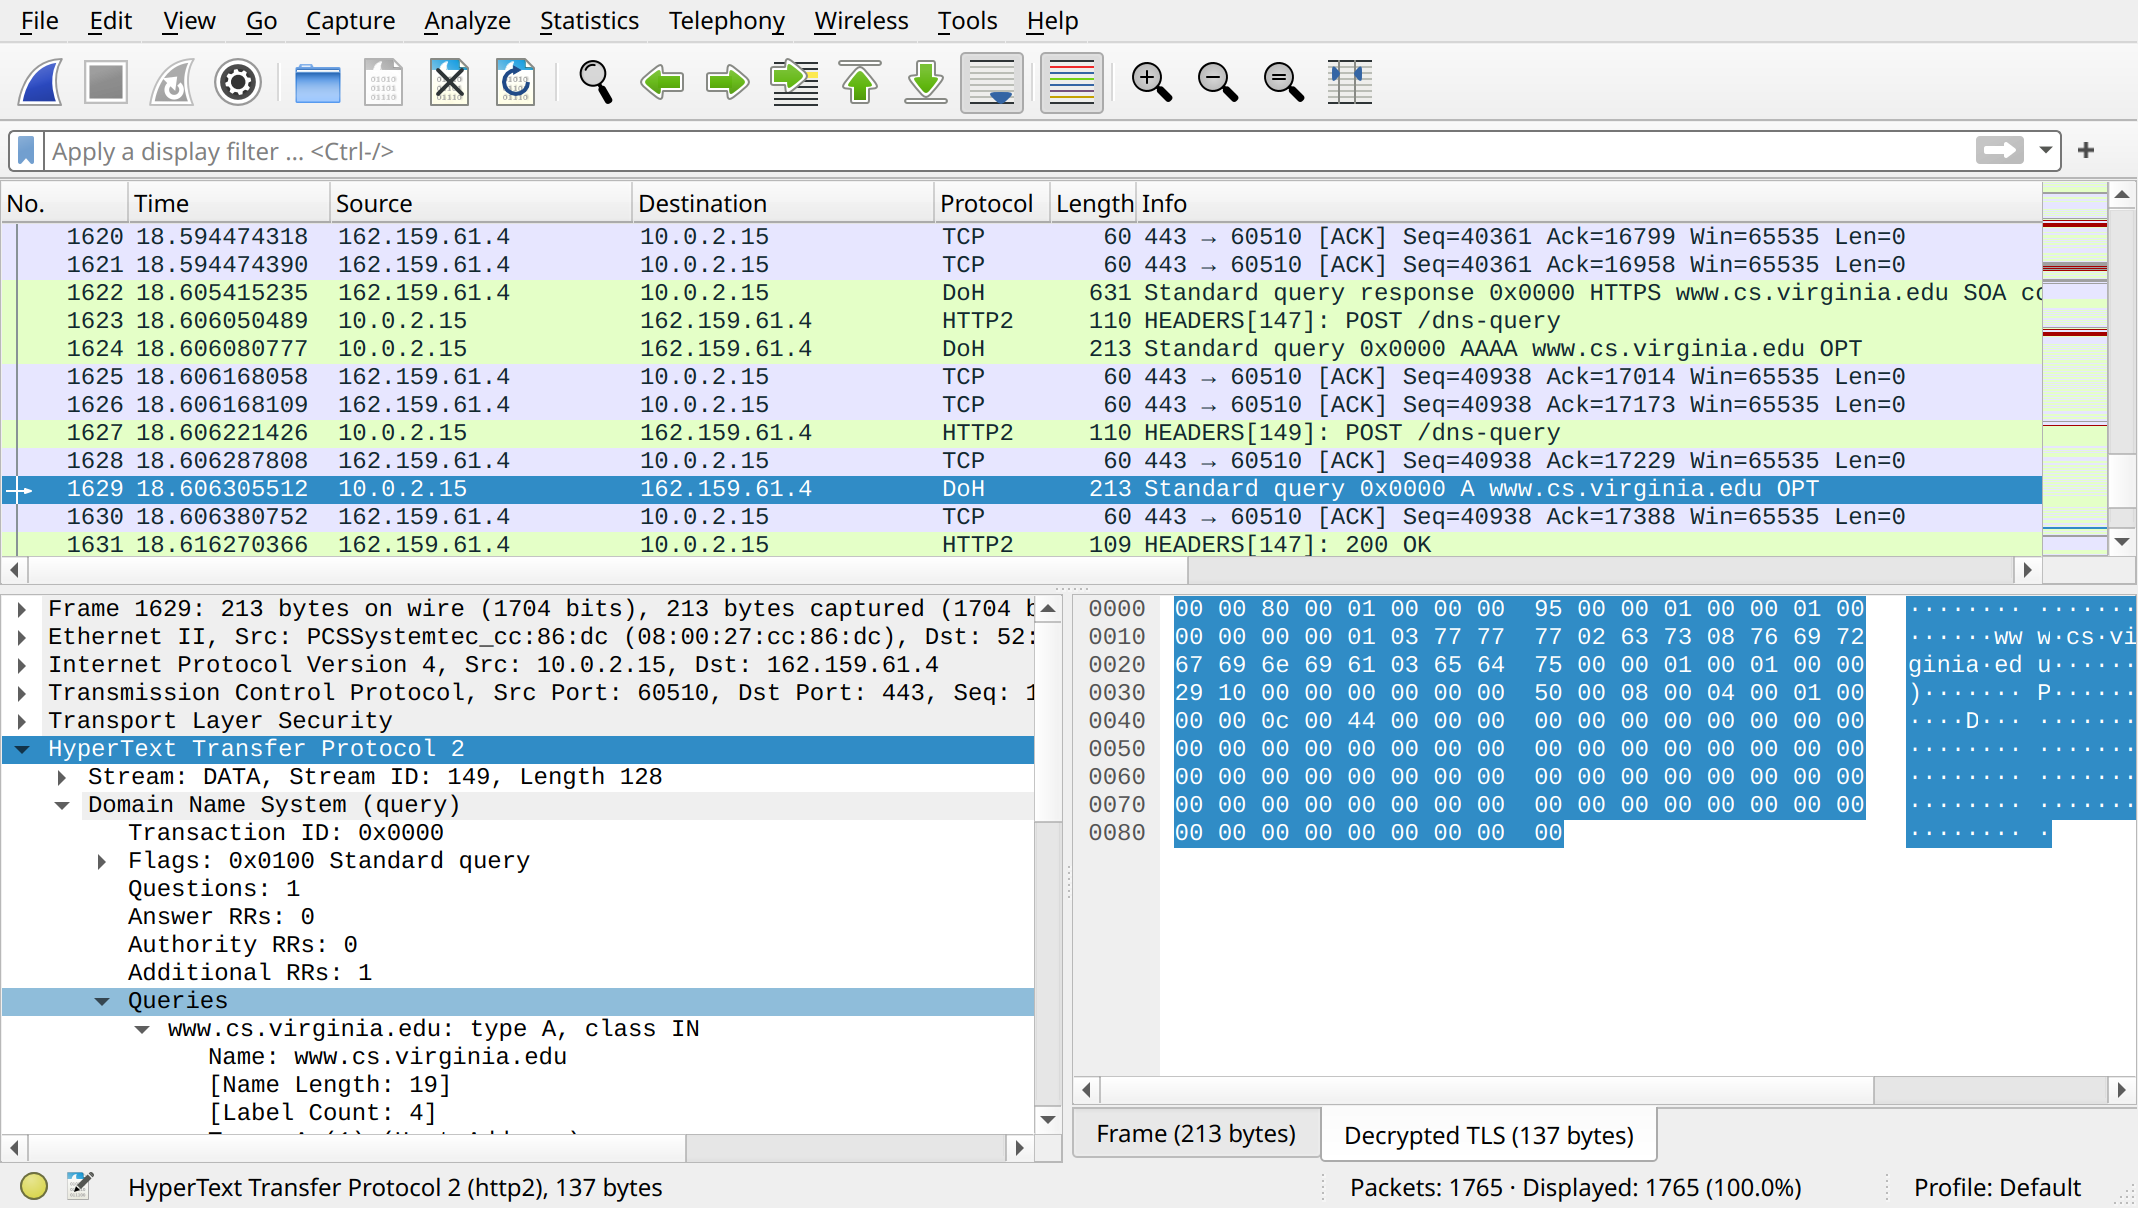
\includegraphics[width=\textwidth]{../intro/wireshark-hi-http.png}}%
\only<12-13>{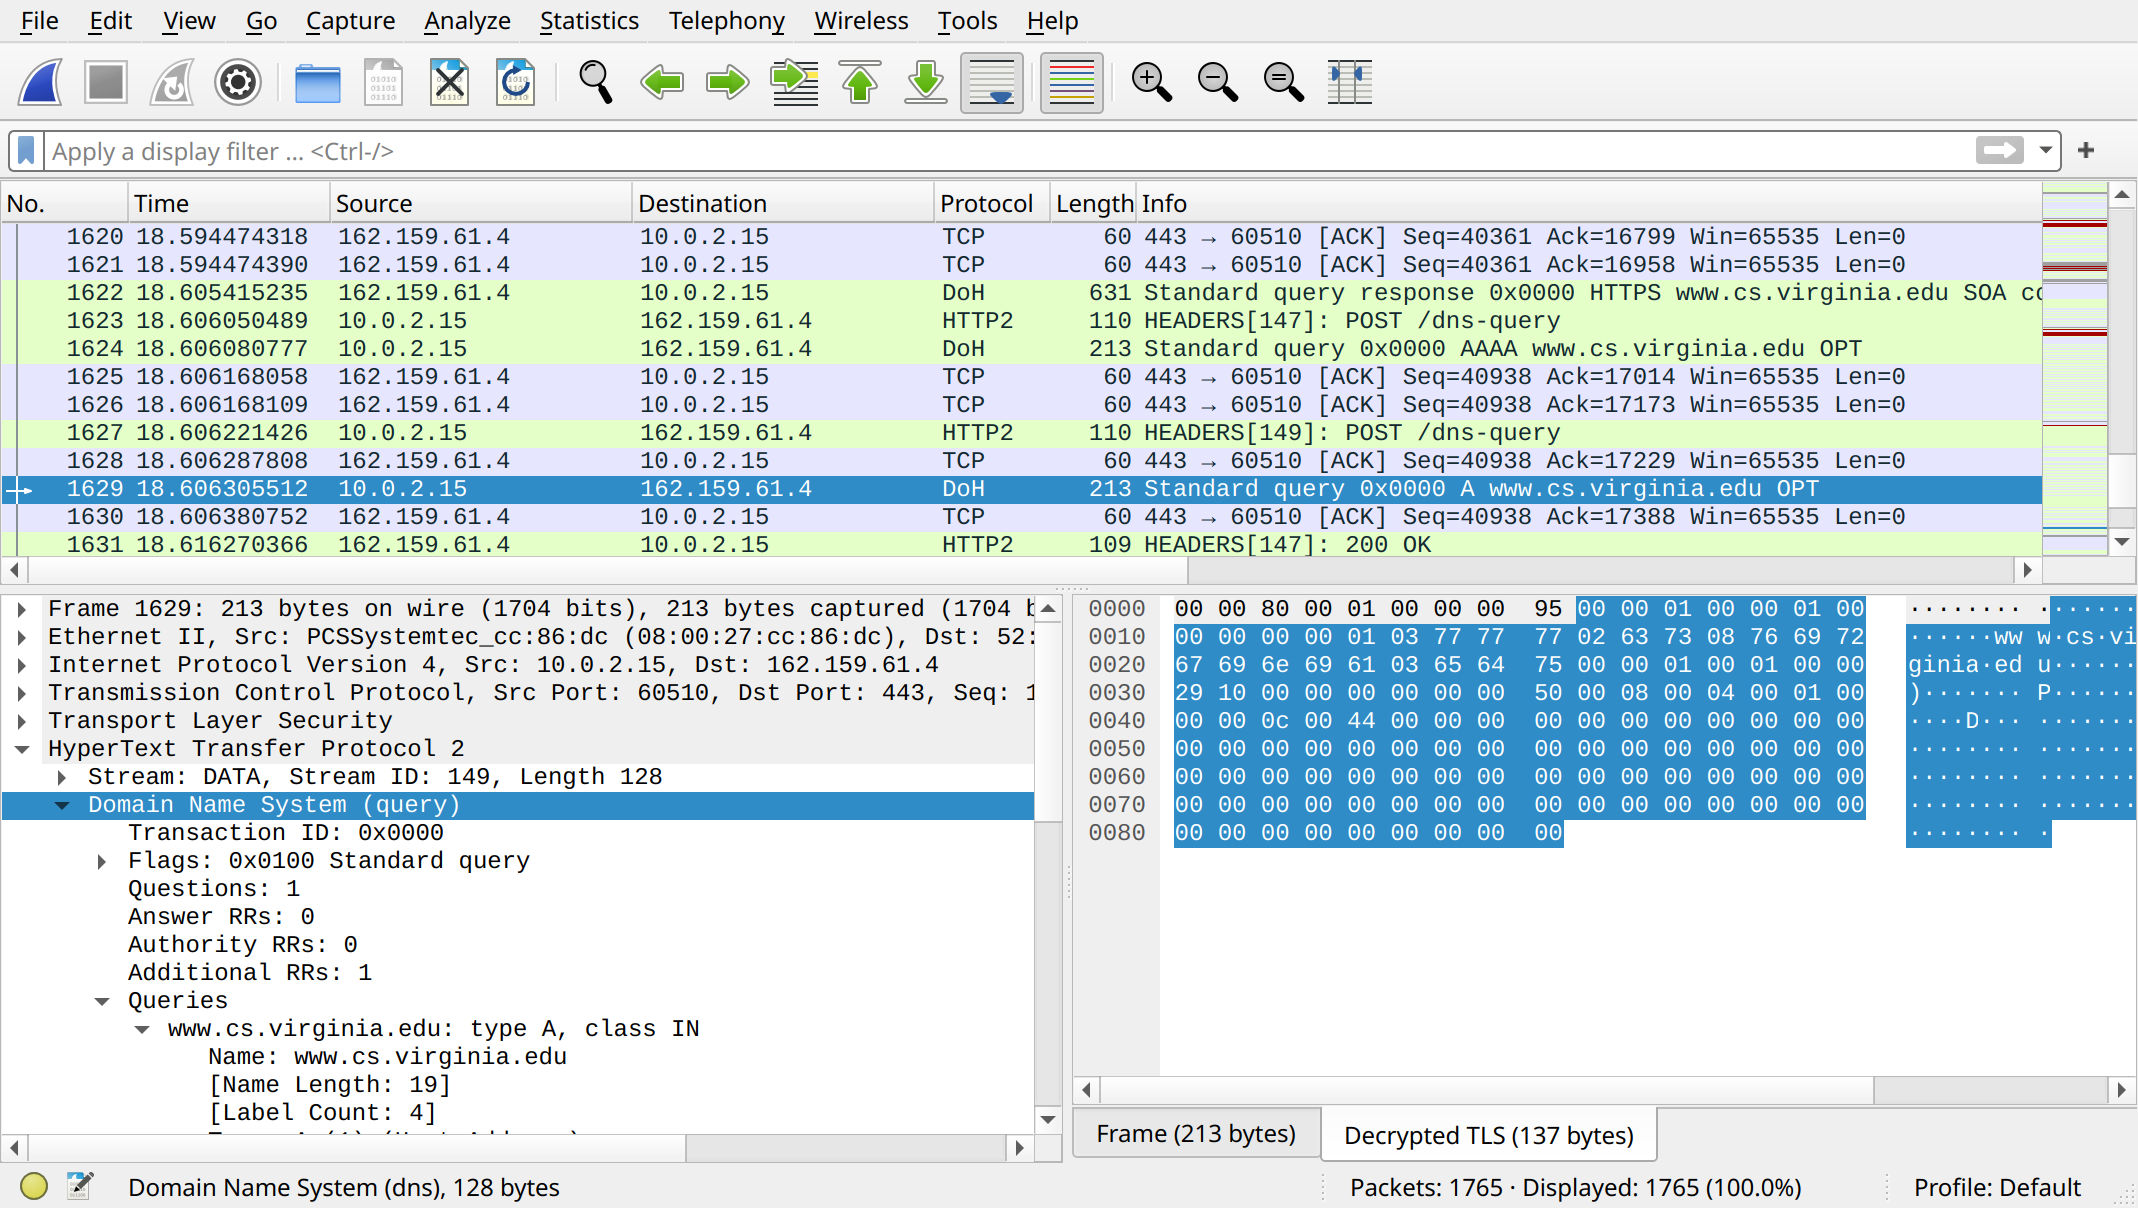
\includegraphics[width=\textwidth]{../intro/wireshark-hi-dns-in-tls.png}}%
};
%\draw[overlay,help lines] (0, 0) grid (14, -8);
\path (0, 0) rectangle (14.5, -7); % for bounding box

\begin{visibleenv}<1> % ethernet
    \doHiliteOneDataLine{1}{2}{0}{0}{4.2}{0}
\end{visibleenv}
\begin{visibleenv}<3> % IP
    \doHilite{2}{3}{4.2}{0}{0.5}{2}
\end{visibleenv}
\begin{visibleenv}<5> % TCP
    \doHilite{3}{4}{0.5}{2}{1.7}{3}
\end{visibleenv}
\begin{visibleenv}<7> % TLS
    \doHilite{4}{5}{1.7}{3}{1.4}{12}
\end{visibleenv}
\begin{visibleenv}<9> % HTTP, decrypted TLS
    \path[draw,red,very thick] (8.9, -7.5) rectangle (11.3, -7.9);
    \node[align=left,overlay box,anchor=south] at (10.4, -7.5) {
        setup step: got Firefox to output \\
        cryptographic keys ({\fontsize{10}{11}\selectfont using \tt SSLKEYLOGFILE})
    };
\end{visibleenv}
\begin{visibleenv}<10> % HTTP
    \doHilite{5}{6}{0}{0}{2.69}{8}
\end{visibleenv}
\begin{visibleenv}<12> % DNS
    \doHilite{7}{8}{2.7}{0}{2.69}{8}
\end{visibleenv}
\end{tikzpicture}
\end{frame}

% FIXME: show multiple related packets --- emphasize filter window
\begin{frame}{}
\begin{tikzpicture}
\tikzset{
    overlay box/.style={fill=white,fill opacity=0.9}
}
\node[overlay,anchor=north west,inner sep=0mm] (base) at (0, 0) {
    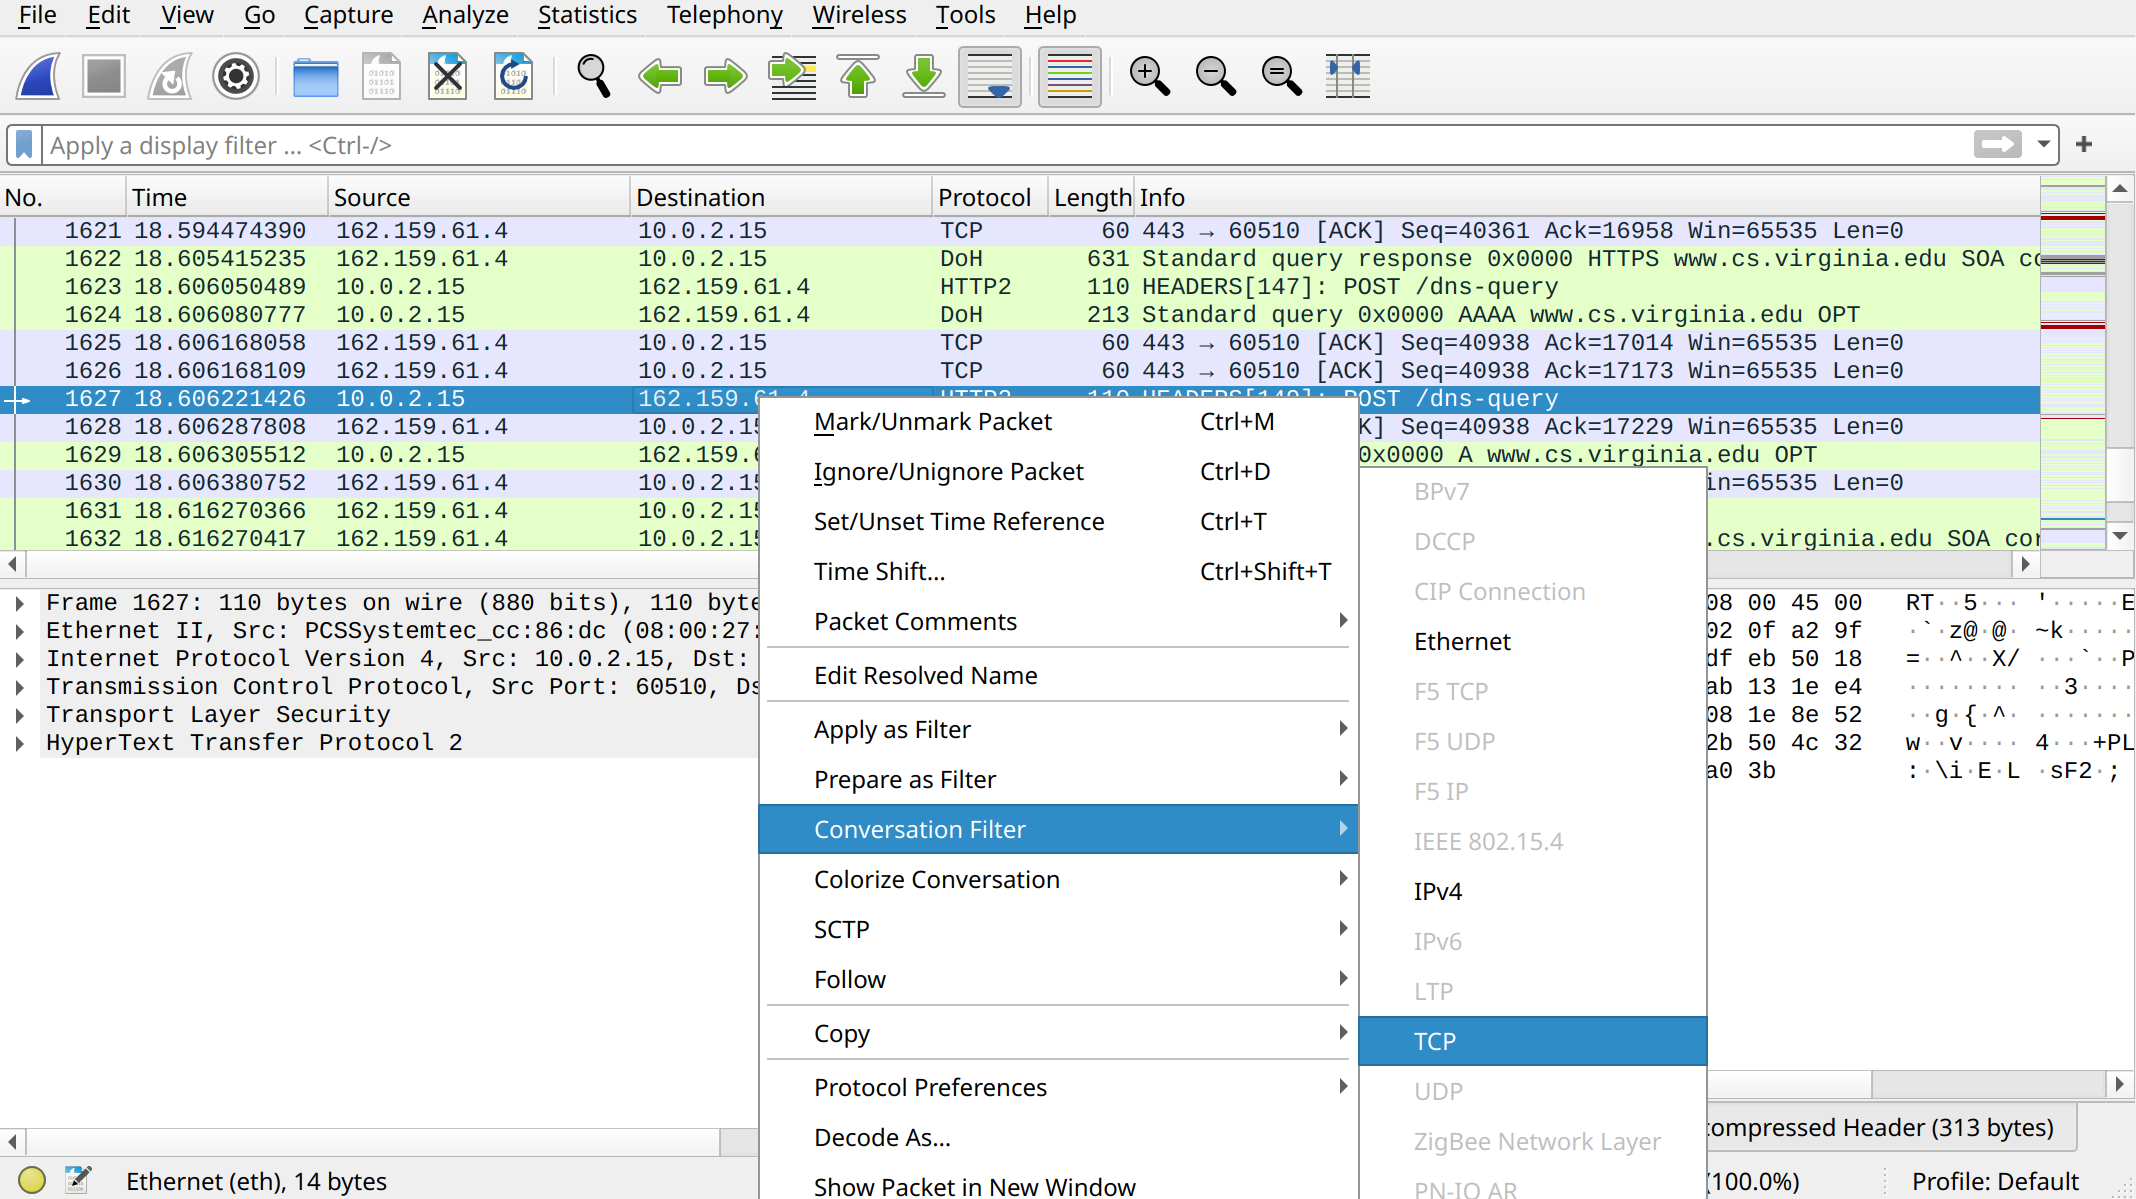
\includegraphics[width=\textwidth]{../intro/wireshark-menu-tcp-filter.png}
};
\path (0, 0) rectangle (14.5, -7); % for bounding box
\end{tikzpicture}
\end{frame}

\begin{frame}{}
\begin{tikzpicture}
\tikzset{
    overlay box/.style={fill=white,fill opacity=0.9}
}
\node[overlay,anchor=north west,inner sep=0mm] (base) at (0, 0) {
    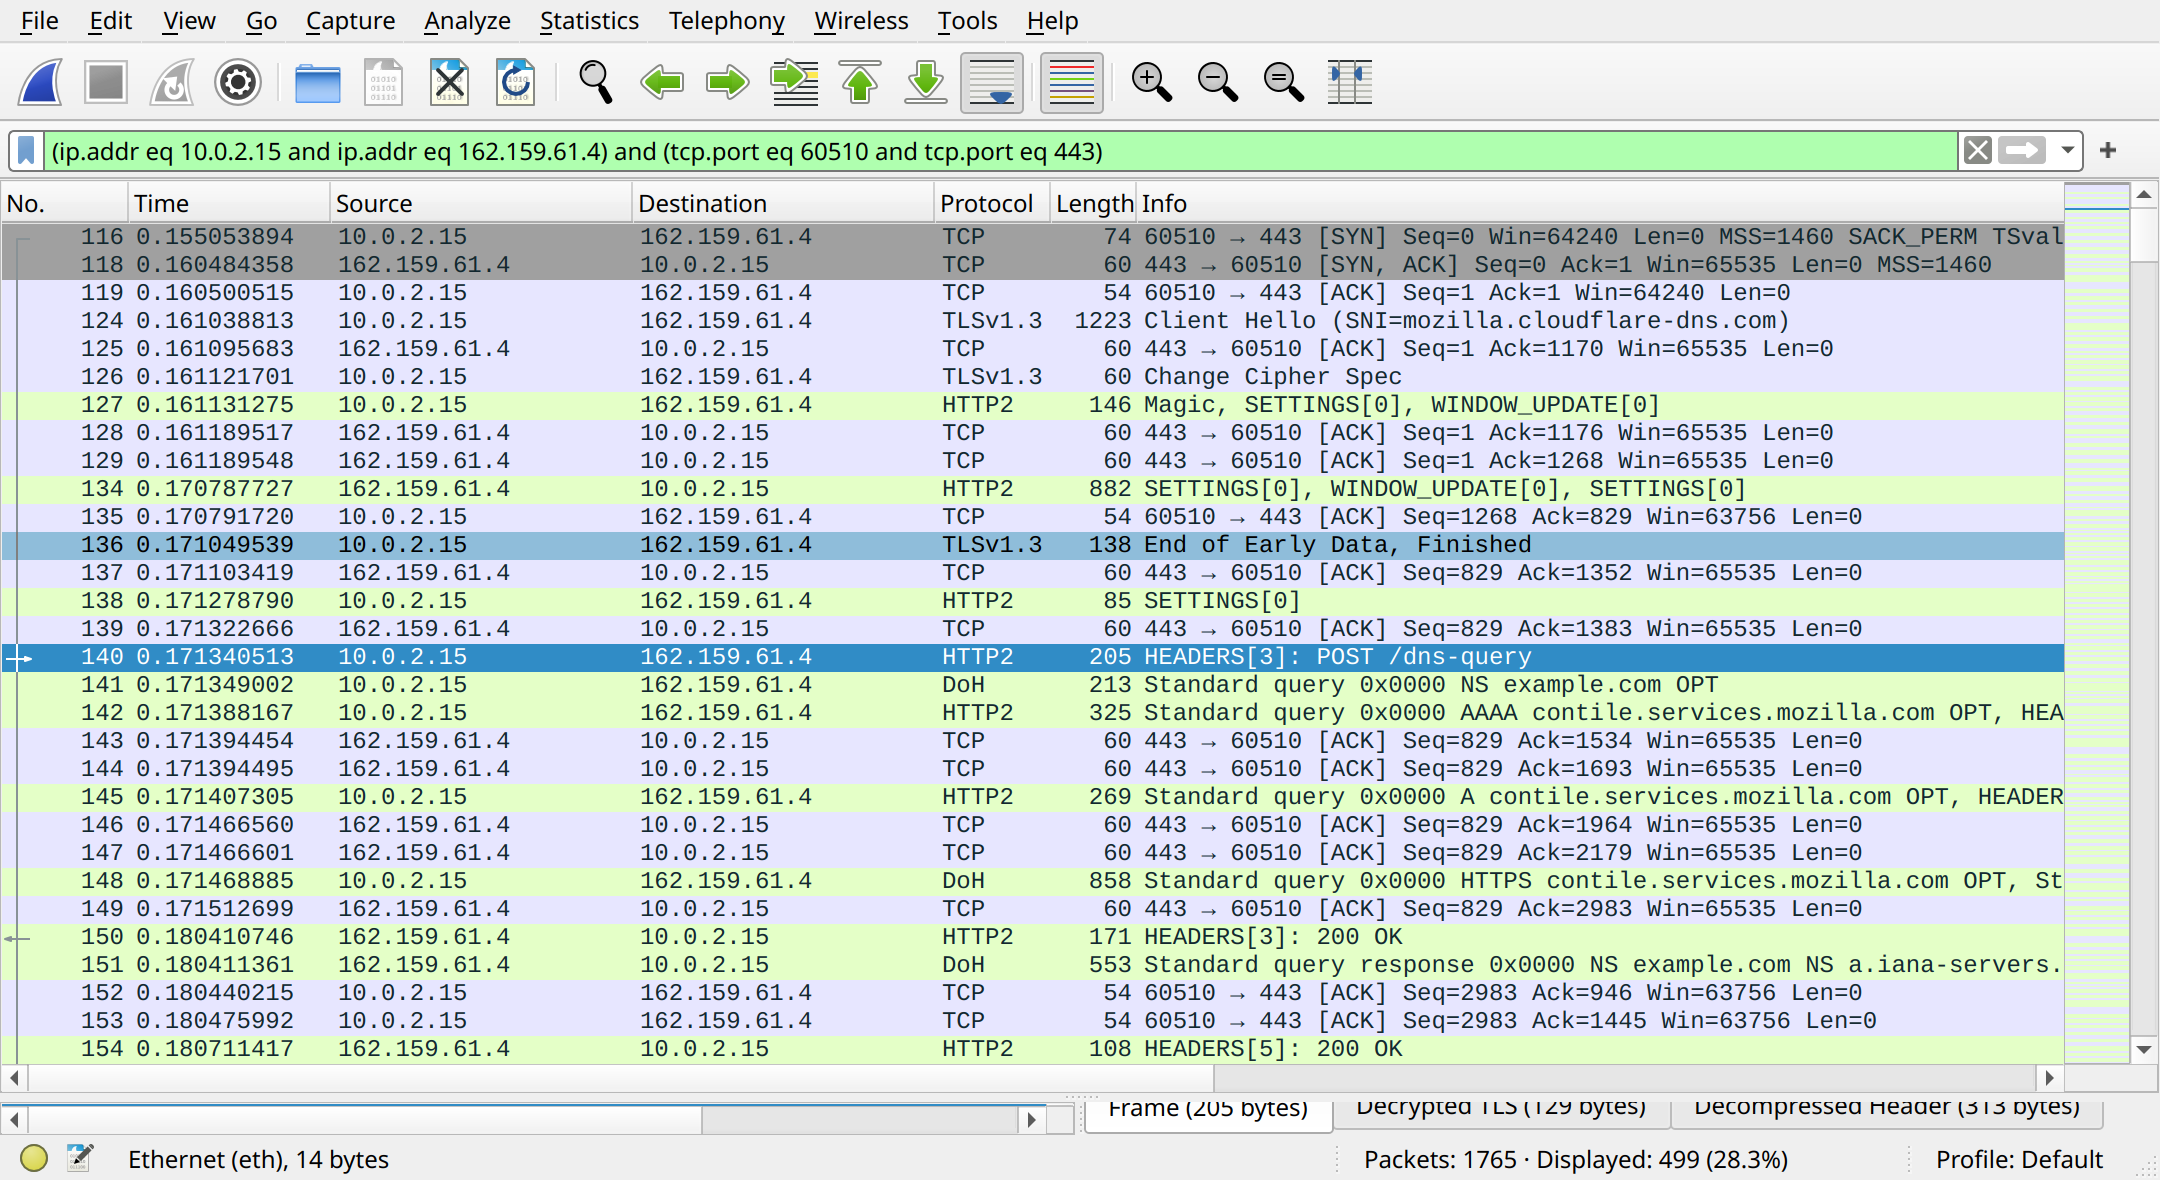
\includegraphics[width=\textwidth]{../intro/wireshark-filtered.png}
};
\path (0, 0) rectangle (14.5, -7); % for bounding box
%\draw[overlay,help lines] (0, 0) grid (14, -8);
%\draw[overlay,help lines,dotted] (0, 0) grid[step=0.2] (14, -8);
\begin{visibleenv}<1>
    \path[draw, red, very thick] (0.3, -0.9) rectangle (13.15, -1.15);
    \node[anchor=north,overlay box,text=red] (filter expr label) at (6.5, -1.15) {
        filter expression 
    };
    \node[anchor=north,overlay box,font=\fontsize{10}{11}\selectfont,align=left] at (filter expr label.south) {
        based on address ($\sim$ machine) and port number ($\sim$ program/socket) fields  \\
        usually means all part of one socket connection
    };
    \path[draw, red, very thick] (10.3, -7.6) rectangle (12.1, -7.9);
    \node[anchor=south,overlay box,text=red] at (11.4, -7.6) {
        499 packets in ``conversation''
    };
\end{visibleenv}
\begin{visibleenv}<2>
    \path[draw,red, very thick] (0, -1.9) rectangle (.85, -2.24);
    \path[draw,red, very thick] (0, -3) rectangle (.85, -3.37);
    \node[overlay box,anchor=west,text=red] at (.85, -2.5) {
        some packets not shown from filter
    };
\end{visibleenv}
\begin{visibleenv}<3>
    \path[draw,red,very thick] (6.25, -1.47) rectangle (7.1, -7.2);
    \node[align=left,overlay box,anchor=south east,text=red] at (6.25, -3) {
        highest layer used \\
        in each packet
    };
    \node[align=left,overlay box,anchor=north east,text=black,font=\fontsize{10}{11}] at (6.25, -3) {
        connection only `for' \\
        DNS over HTTPS (DoH) \\
        but many packets \\
        only needed for \\
        bookkeeping for \\
        the `lower' layers
    };
\end{visibleenv}
\begin{visibleenv}<4>
    \path[draw,red,very thick] (2.2, -1.47) rectangle (6.25, -7.2);
    \node[align=left,overlay box,anchor=west] at (6.25, -4) {
        bookkeeping packets sent \\
        in both directions
    };
\end{visibleenv}
\end{tikzpicture}
\end{frame}


\subsection{end-to-end argument}
\begin{frame}<1>[label=endToEndStatement]{end-to-end argument}
    \begin{itemize}
    \item Saltzer, Reed, Clark, ``End-to-End Arguments in System Design''
    \item ``The function in question can completely and correctly be implemented 
    \myemph<2>{only with the knowledge and help of the application standing at the end points} of the communication
    system. Therefore, providing that questioned function as a feature of the communication
    system itself is not possible. (Sometimes 
    \myemph<3>{an incomplete version of the function provided by the communication system may be useful as a performance enhancement}.)''
    \end{itemize}
\end{frame}

\againframe<2>{endToEndStatement}

\begin{frame}{example: reliable file transfer}
    \begin{itemize}
    \item want to make sure correct data transferred
    \vspace{.5cm}
    \item want to protect against:
        \begin{itemize}
        \item \myemph<2>{error in hardware/software on sending machine reading file}
        \item \myemph<2|3>{bits being flipped in memory on forwarding machine}
        \item communication system flipping bits in data
        \item \myemph<2>{hosts crashing during communication}
        \end{itemize}
    \vspace{.5cm}
    \item<2-> \myemph<2>{\it communication system can't help a lot of these things}
    \item<3-> \myemph<3>{\it authors experienced router with bad memory/processor}
    \end{itemize}
\end{frame}

\begin{frame}{solution: end-to-end checks}
    \begin{itemize}
    \item want reliable transfer: compare final files (with hash or similar)
    \vspace{.5cm}
    \item ``end-to-end'' --- doesn't care what middle systems do
    \end{itemize}
\end{frame}


\againframe<3>{endToEndStatement}

\begin{frame}{end-to-end in practice}
    \begin{itemize}
    \item ``narrow waist'' of IP doesn't provide many gaurnetees
        \begin{itemize}
        \item no gaurentees about reliable transmission, duplicate suppression, message order, \ldots
        \end{itemize}
    \item but try to provide good service (``best effort'')
    \vspace{.5cm}
    \item in design: typically middle systems won't know/care about what's forwarded
        \begin{itemize}
        \item but many exceptions
        \end{itemize}
    \end{itemize}
\end{frame}


\subsection{end-to-end exercise}
\begin{frame}{exercise}
\begin{itemize}
    \item which idea is most/least consistent with end-to-end principle?
    \item A. having switches send a signal to the sending end-host when it drops their packets
    \item B. an end-host sending a message to two different switches so it's more likely to reach its destination
    \item C. an end-host telling a switch when it's received a packet, so the switch can avoid resending it
    \item D. an end-host indicating whether its packets should be dropped if they cannot be forwarded quickly
\end{itemize}
\end{frame}


